% $Id: INF_Diplomarbeit.tex 1660 2010-02-25 13:57:42Z tkren $
%
% TU Wien - Faculty of Informatics
% thesis template
%
% This template is using the memoir document class, see
% <http://www.ctan.org/tex-archive/macros/latex/contrib/memoir/memman.pdf>
% <http://www.ctan.org/info/latex-samples/MemoirChapStyles/MemoirChapStyles.pdf>
%
% For questions and comments send an email to
% Thomas Krennwallner <tkren@kr.tuwien.ac.at>
%

								
\documentclass[a4paper,12pt, oneside]{memoir}
%\chapterstyle{veelo}
\usepackage{graphicx} 
\usepackage{placeins}
\usepackage{caption}


\chapterstyle{madsen}
\setlength{\parskip}{6pt plus 1pt minus 1pt}
\setlength{\parindent}{0pt}

\usepackage{TUINFDA}

\thesistitle{Cluster visualization for interactive maps}
\thesisdate{\the\day.\the\month.\the\year}

\thesisdegree{Diplom-Ingenieur}
\thesiscurriculum{Software Engineering and Internet Computing}
\thesisverfassung{Verfasser}
\thesisauthor{Josef Dabernig}
\thesismatrikelno{0927232}
% \thesisauthoraddress{} % your address

\thesisbetreuung{Betreuer}
\thesisbetreins{Prof.~Dr.~Silvia Miksch}
\thesisbetrzwei{Univ.-Ass.~Dr. Amin Anjomshoaa}

\newcommand{\EnableCustomThesisLayout}{
\setheaderspaces{*}{1.5cm}{*}
}

\usepackage{multirow}
\usepackage{rotating}

\begin{document}


% the front matter                                                 
\frontmatter

% $Id: titlepage.tex 2165 2010-08-07 04:42:52Z tkren $
%
% TU Wien - Faculty of Informatics
% thesis titlepage
%
% This titlepage is using the geometry package, see
% <http://www.ctan.org/macros/latex/contrib/geometry/geometry.pdf>
%
% For questions and comments send an email to
% Thomas Krennwallner <tkren@kr.tuwien.ac.at>
%

% setup page dimensions for titlepage
\newgeometry{left=2.4cm,right=2.4cm,bottom=2.5cm,top=2cm}

% force baselineskip and parindent
\newlength{\tmpbaselineskip}
\setlength{\tmpbaselineskip}{\baselineskip}
\setlength{\baselineskip}{13.6pt}
\newlength{\tmpparindent}
\setlength{\tmpparindent}{\parindent}
\setlength{\parindent}{17pt}
\newlength{\tmpparskip}
\setlength{\tmpparskip}{\parskip}
\setlength{\parskip}{0pt}


% first titlepage
\thispagestyle{tuinftitlepage}

%
% Kludge: for each titlepage set \pagenumbering to a different
% style. This is used to fix a problem with hyperref, because there
% are multiple "page 1" and hyperref hates that
%
\pagenumbering{Alph}

\begin{center}
%
\begin{minipage}[t][5.2cm][b]{\linewidth}%
    \centering%
    %\renewcommand{\baselinestretch}{0.9} % very long titles need to tweak baselinestretch...
    \thesistitlefontHUGE\sffamily\bfseries\tuinfthesistitle%
\end{minipage}


\vspace{1.3cm}

{\thesistitlefontLARGE\sffamily \tuinfthesistype}

\vspace{6mm}

% {\thesistitlefontlarge\sffamily zur Erlangung des akademischen Grades}

\vspace{6mm}

% {\thesistitlefontLARGE\sffamily\bfseries \tuinfthesisdegree}

\vspace{6mm}

% {\thesistitlefontlarge\sffamily im Rahmen des Studiums}

\vspace{6mm}

% {\thesistitlefontLarge\sffamily\bfseries \tuinfthesiscurriculum}

\vspace{6.5mm}

% {\thesistitlefontlarge\sffamily eingereicht von}

\vspace{6mm}

{\thesistitlefontLarge\sffamily\bfseries \tuinfthesisauthor}

\vspace{1.5mm}

{\thesistitlefontlarge\sffamily Matrikelnummer \tuinfthesismatrikelno} 

\vspace{1.5cm}

\begin{minipage}[t][1.7cm][t]{\textwidth}%
  \vspace{0pt}\raggedright\thesistitlefontnormalsize\sffamily
  %
  an der

  Fakult\"{a}t f\"{u}r Informatik der Technischen Universit\"{a}t Wien
\end{minipage}

\begin{minipage}[t][4cm][t]{\textwidth}%
  \vspace{0pt}\sffamily\thesistitlefontnormalsize\raggedright
  %
  Betreuung

  \tuinfthesisbetreuung: \tuinfthesisbetreins

%  \raggedright Mitwirkung: \tuinfthesisbetrzwei

\end{minipage}

% we want a german date, then switch back to english
 \selectlanguage{ngerman}
 \begin{minipage}[t][2cm][t]{\textwidth}%
  \vspace{0pt}\sffamily\thesistitlefontnormalsize
  \begin{tabbing}%
    Wien, \tuinfthesisdate
    %    \> \begin{minipage}[t][0.5cm][t]{51mm}\centering (Unterschrift \tuinfthesisverfassung)\end{minipage}
%    \> \begin{minipage}[t][0.5cm][t]{51mm}\centering (Unterschrift \tuinfthesisbetreuung)\end{minipage}
    \end{tabbing}
\end{minipage}
\selectlanguage{english}

\end{center}

% we want an empty page right after first titlepage
\cleardoublepage

% we're done with the titlepages, proceed with default pagenumbering
\pagenumbering{roman}

% restore baselineskip
\setlength{\baselineskip}{\tmpbaselineskip}
\setlength{\parindent}{\tmpparindent}
\setlength{\parskip}{\tmpparskip}


% back to normal geometry
\restoregeometry


%%% Local Variables:
%%% TeX-PDF-mode: t
%%% TeX-debug-bad-boxes: t
%%% TeX-parse-self: t
%%% TeX-auto-save: t
%%% reftex-plug-into-AUCTeX: t
%%% End:

\EnableCustomThesisLayout
% \chapter*{Erklärung zur Verfassung der Arbeit}

\tuinfthesisauthor\\
% \tuinfthesisauthoraddress

\vspace*{1.2cm}

Hiermit erkläre ich, dass ich diese Arbeit selbständig verfasst habe, 
dass ich die verwendeten Quellen und Hilfsmittel vollständig angegeben 
habe und dass ich die Stellen der Arbeit - einschließlich Tabellen, 
Karten und Abbildungen -, die anderen Werken oder dem Internet im 
Wortlaut oder dem Sinn nach entnommen sind, auf jeden Fall unter Angabe 
der Quelle als Entlehnung kenntlich gemacht habe.\\



  \begin{tabbing}%
    \hspace{15mm} \= \hspace{65mm} \= \hspace{42mm} \kill
    \> Wien, \tuinfthesisdate \> {\raggedright\rule{51mm}{0.5pt}} \\
    \> \> \begin{minipage}[t][0.5cm][t]{51mm}\centering
 (Unterschrift \tuinfthesisverfassung)\end{minipage}
  \end{tabbing}


%
% abstract
%


\chapter*{Abstract}

This thesis investigates ways of visualization for presenting clustered information on maps. Performance and readability of digital mapping applications decreases when displaying large amounts of data. Clustering can be used to group overlapping items and reduce visual clutter of the map presentation. 

Visualization techniques for putting clusters on a map are researched and evaluated in an exploratory analysis. Existing concepts from visual cluster analysis and geovisualization, as well as established classifications form the foundations of the presented study. \textit{Map types} as well as \textit{cluster visualization techniques} are presented. The \textit{evaluation} classifies the stated techniques for cluster visualization on maps.

The presented map types for visualizing clusters range from standard, \textit{geographic maps} with markers, \textit{Heat maps} to \textit{Dot Grid maps} and a \textit{Voronoi} map. Cluster visualization techniques include \textit{icon-based/glyphs}, \textit{pixel-based}, as well as \textit{geometric/diagrams}. The evaluation of visualization techniques for clusters on a map proposes a custom set of criteria. \textit{Showing the number of items within clusters} is considered as a main feature of simple cluster visualizations on maps. Further, the study identifies \textit{showing cluster areas} and \textit{extra cluster information} as two additional aspects of primary interest when comparing approaches to cluster visualization on maps.   

The results are discussed and put into practice by evaluating the visual aspects of \textit{Geocluster}, a server-side clustering implementation for maps.
\newpage

\setcounter{tocdepth}{3}
\tableofcontents
\newpage

%TODO enable
%\listoffigures
\newpage

%\listoftables
\newpage

%
% start of the thesis
%
\mainmatter
\setcounter{secnumdepth}{3}


%
% intro
%

\chapter{Introduction}

Digital mapping applications on the Internet are strongly emerging. Big players like Google Maps\footnote{\url{https://maps.google.at}} and OpenStreetMap\footnote{\url{http://www.openstreetmap.org/ }} provide online maps, that users can view and interact with. Maps allow telling stories and communicating data in a visual way. They can be used to get a quick overview of points-of-interest in a certain area. If a large amount of information is contained in such an area, visual clutter is causing problems. Obviously, when telling a story, information needs to be told in a compact way as the human brain can only process a limited amount of data at the same time~\cite{noellenburg11geovis, Delort10vis}.

Clustering\footnote{\url{http://en.wikipedia.org/wiki/Cluster_analysis}} is a technique for grouping objects with similarities that can be used to reduce visual clutter as described before. Clustering points on a map enhances performance and readability of data-heavy map applications. Client-side clustering uses JavaScript to group overlapping items. Server-side clustering is needed when too many items slow down processing and create network bottle necks. This paper aims at discussing visual aspects of Geocluster, a server-side clustering implementation for maps. It considers well-separated, spatial clusters based on Euclidean distance.

The primary goal is to evaluate cluster visualization techniques for creating interactive maps based on large data sets. Visual ways for presenting clustered data on maps should be researched and summarized. Combining existing concepts from visual cluster analysis and geovisualization should provide a better understanding of theoretic backgrounds and put into context. The idea is to draw practical conclusions from the overlap of these two complex areas of research. Given the lack of existing publication on visualizing clusters on maps for reference, the study rather aim at exploration of concepts and ideas than being a complete reference. 


\section{Structure}

The given introduction is expanded by a discussion of \textit{related work} in the field of geovisualization and visual cluster analysis. In addition, the \textit{methods} being used to achieve the goal evaluating cluster visualization techniques for interactive maps.

Chapter \ref{chapter:foundations} describes the theoretic \textit{foundations} being researched. Basic concepts of geovisualization as visual variables, visual data exploration techniques and clutter reduction are explained.

Chapter \ref{chapter:results} discusses the main \textit{results} of the study. Map visualization types, as well as cluster visualization techniques are explained and summarized within an exploratory evaluation.

Chapter \ref{chapter:discussion} is a \textit{discussion} of the previously presented results and applies the evaluation of cluster visualization techniques for maps to the practical use case of Geocluster.

Chapter \ref{chapter:conclusion} finalizes the paper by drawing \textit{conclusions} of the presented results and discussion.


\section{Related work}

While many publications have been found on either cluster analysis or geovisualization, few of them touch upon both subjects at the same time. There hasn't been found any study that compares the different techniques for visualizing clusters on maps as its primary goal.

A primary resource instead are publications on individual approaches for cluster geovisualization: 
Heat maps \cite{geotree, hotmap}, Voronoi Diagrams \cite{Delort10vis, voromap}, Convex Hulls \cite{Cristani08geoimagemaps}. A well research blog article talks about different ways to visualize clusters on maps~\cite{web:clustering-google}. A more complex visualization is provided by Bristle Maps \cite{bristle}. Various cluster visualization techniques on maps are combined in \cite{andrienko2012sca}. Self-organizing maps represent clustered information in virtual space \cite{som}.

On a practical note, Leaflet.markercluster\footnote{\url{https://github.com/Leaflet/Leaflet.markercluster}}, the OpenLayers Cluster Strategy\footnote{\url{http://openlayers.org/dev/examples/strategy-cluster.html}} and MarkerClusterer for Google Maps\footnote{\url{http://google-maps-utility-library-v3.googlecode.com/svn/trunk/markerclusterer/docs/reference.html}} are common implementations for client-side clustering that visualize clusters on maps.

For classification of the researched techniques, 3 taxonomies have been considered. ``Visual variables'' by Jacques Bertin \cite{bertin67graphics, bertin83graphics} with some adjustments by Alan M. MacEachren \cite{MacEachren95maps} and Leland Wilkinson \cite{Wilkinson05grammar}. ``Classification of visual data exploration techniques'' by Daniel A. Keim~\cite{keim2001vis} and the ``Clutter Reduction Taxonomy'' by Geoffrey Ellis and Alan Dix~\cite{ellis08clutter}. Further, related taxonomies are found \cite{lohse, shneiderman}.
 
In addition, publications on cluster and multi-variate data visualization techniques \cite{ward02glyphs, zhang07thesis, ElmqvistDGHF08, hiervis}, geovisualization \cite{noellenburg11geovis, maceachren-geovis, MacEachren07cartovis} and diagrams \cite{ladenhauf12dia} are extensive resources for the individual topics being discussed in this paper.



\section{Method}

Scientific publications as well as real-world implementations have been researched in order to get a good overview of existing technologies related to visualizing clusters on maps. Given the lack of comparative publications in that particular field, papers on the individual topics of visualization, geovisualization and cluster analysis have been compared for overlapping concepts. As no fixed criteria, despite the general context and goals of the paper have been set, the research was mainly conducted in an explorative way. The criteria of published classifications and taxonomies have been reviewed to match the use case for visualizing clusters on web maps.

Based on an overview of foundations in geovisualization and cluster analysis, the main part of the study tries to enumerate the diverse approaches for visualizing clusters on maps. This is done from two perspectives: \textit{map visualization types} cover the whole visualization and \textit{cluster visualization techniques} focus on individual clusters being represented on maps. Finally, an attempt for classification has been made as part of evaluation based on exploratory analysis: custom criteria derived from existing taxonomies are defined and the researched technologies get classified amongst those criteria.









%
% foundations - vis
%

\chapter{Foundations}
\label{chapter:foundations-vis}

In the following chapter, foundations for visualizing clusters on a map will be discussed. Basics of geographic visualization and their driving forces lead to abstraction and clustering as a tool for simplifying information on maps. Visual variables, as well as classification approaches for geovisualization will be reviewed in order to discuss existing concepts for displaying aggregated data on a map.

Visualization is driven by the basic belief that `seeing' is a good way of understanding and generating knowledge. Humans have a very well developed sense of sight, a fact which is underlined by more of 50 percent of the neurons in our brain being used for vision.~\cite{vislecture}. 

MacEachren \& Kraak~\cite{maceachren-geovis} define that ``Geovisualization integrates approaches from visualization in scientific computing (ViSC), cartography, image analysis, information visualization, exploratory data analysis (EDA), and geographic information systems (GISystems) to provide theory, methods, and tools for visual exploration, analysis, synthesis, and presentation of geospatial data (any data having geospatial referencing).'' In his lecture notes on ``Geographic visualization'', Martin N\"{o}llenburg adds that more human-centered definitions exist and observes that the user's needs have to be taken into account for effective geovisualization techniques~\cite{noellenburg11geovis}.


The \textbf{goals of geovisualization} can be summarized using the \textit{map use cube} by MacEachren and Kraak \cite{MacEachren07cartovis}, which is illustrated in figure \ref{fig:geovis-cube}. The goals \textit{exploration, analysis, synthesis and presentation} are classified amongst three dimensions:

\begin{itemize}

\item The type of \textit{task} varies from \textit{knowledge construction} to \textit{information sharing}. While the first is about revealing unknowns and constructing new knowledge, the latter will primarily share existing knowledge.

\item The amount of \textit{interaction} ranges from \textit{high} to \textit{low}. A low level of interaction means a rather passive consumption of knowledge, instead a high level will allow the user to actively influence the visualization.

\item The \textit{users} of visualization are classified between \textit{public} and \textit{private} audiences. A single, private user with specialized skills might require different visualization techniques than large, public audiences.

\end{itemize}

In the given model of the map use cube, the goals of exploring, analyzing, synthesizing and presenting shift between the extremes of the three defined aspects. The first goal of exploring is classified as a task of knowledge construction, based on high interaction and targeted at a rather private audience. On the other hand, presenting is a task of information sharing that requires a low amount of interaction but is suitable for public audiences~\cite{noellenburg11geovis}.  

\begin{figure}[h]
  \begin{center}
    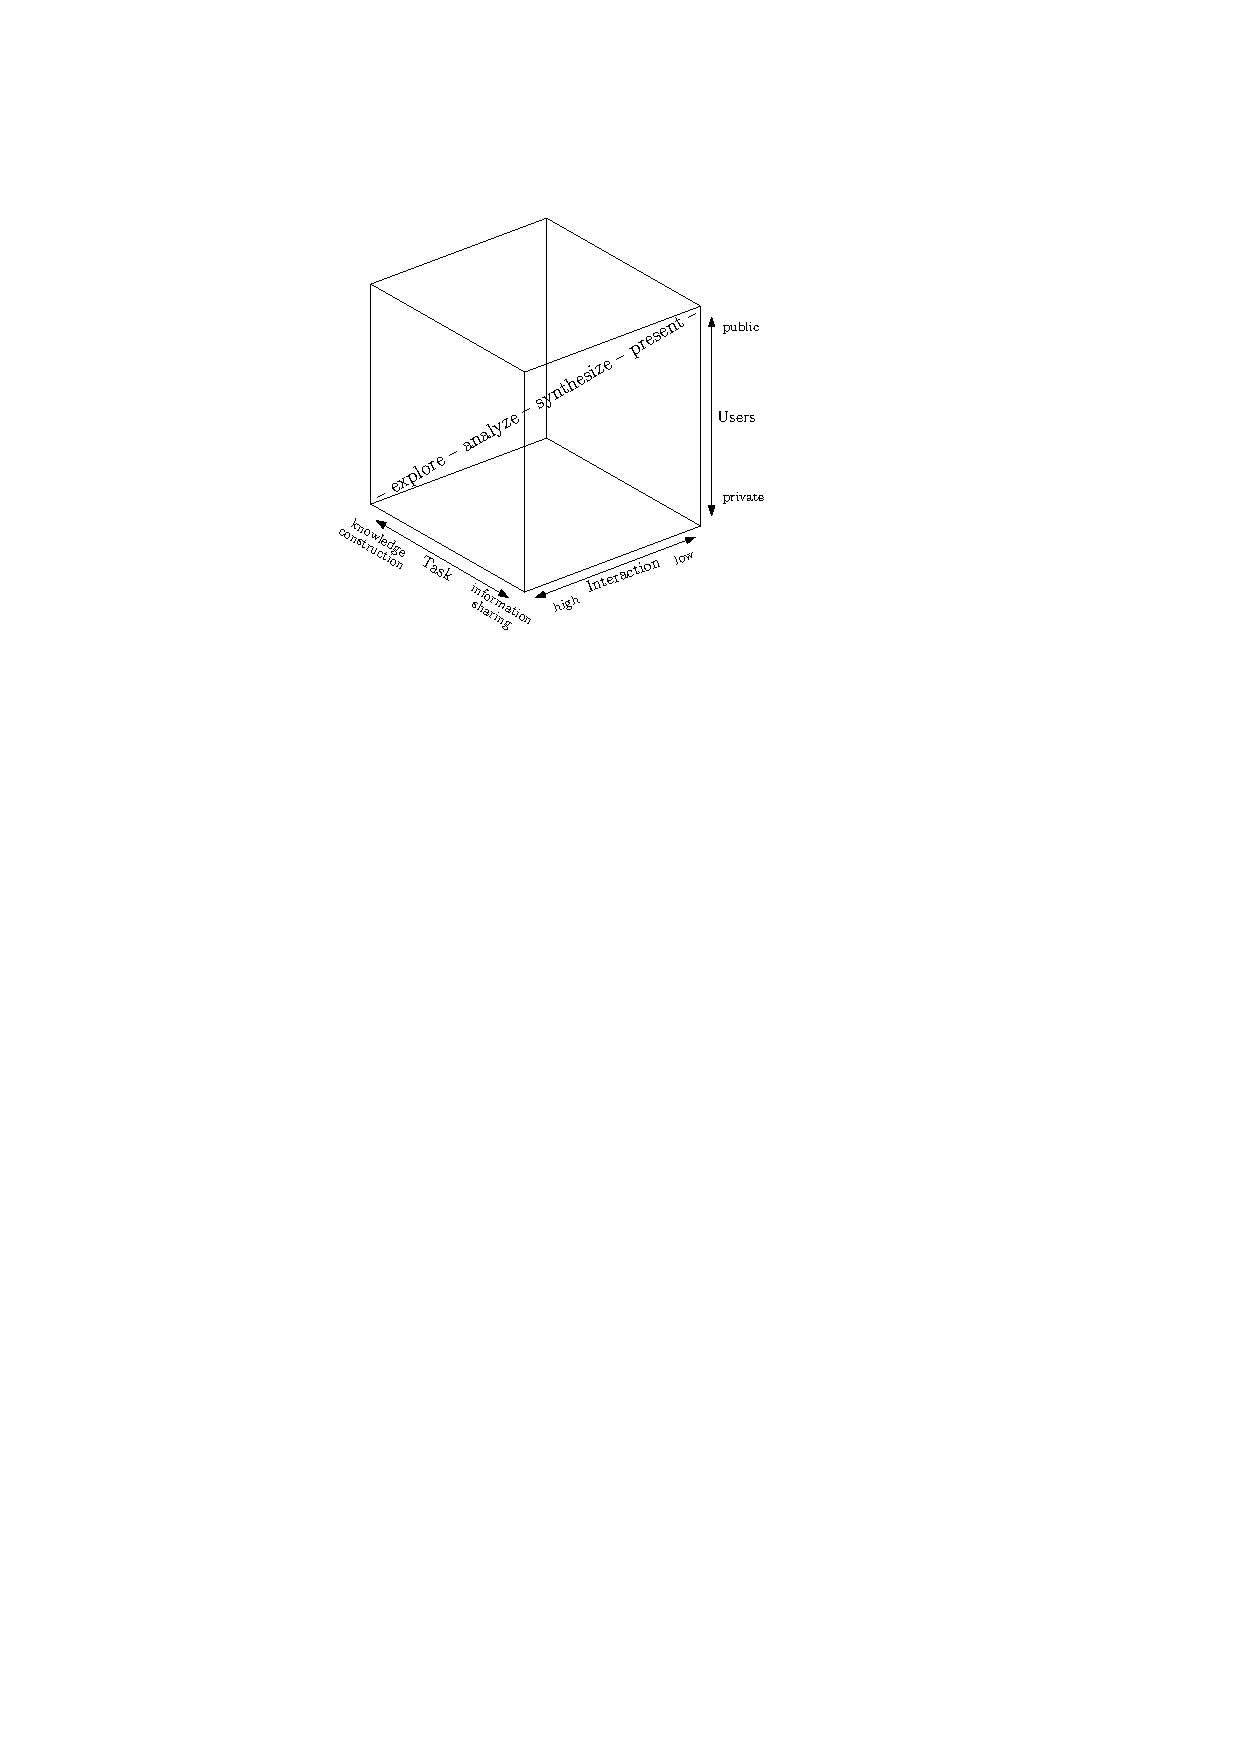
\includegraphics[width=0.65\textwidth]{figures/geovis_goals.pdf}
    \caption{The map use cube after MacEachren and Kraak \cite{MacEachren07cartovis} characterizing geovisualization goals in a three-dimensional space by their level of interaction, their audience, and the addressed tasks.~\cite{noellenburg11geovis}.}
    \label{fig:geovis-cube}
  \end{center}
\end{figure}


Cognitive aspects of visualization help us understand, how visual thinking works. Complex input is abstracted on the retina of the human eye and matched against a vast collection of patterns from experience. Despite generating realistic images, visualization can help generate new ideas by using abstraction to communicate patterns. The idea is to allow the user to join insight, draw conclusions and interact with the data by presenting it in a visual form that reduces the cognitive work needed to perform a given task~\cite{MACEACHREN90apattern, keim2001vis, noellenburg11geovis}. 

Various scientific publications~\cite{phillips82clutter, MACEACHREN90apattern, keim2001vis, harvey2008primer, ellis08clutter, Delort10vis, noellenburg11geovis} that have been researched for this thesis mention the importance of using abstraction for efficiently visualizing information. Especially maps can only highlight interesting information by filtering out unnecessary details of the environment. For example, a road map is better visualized on a clear background instead of satellite images that would distract the user from the primary goal of finding directions. The challenge is to balance realism and abstraction in geovisualization depending on the problem~\cite{noellenburg11geovis}.

\newpage
\section{Visual variables}
\label{chapter:vis-variables}

\begin{figure}[h]
  \begin{center}
    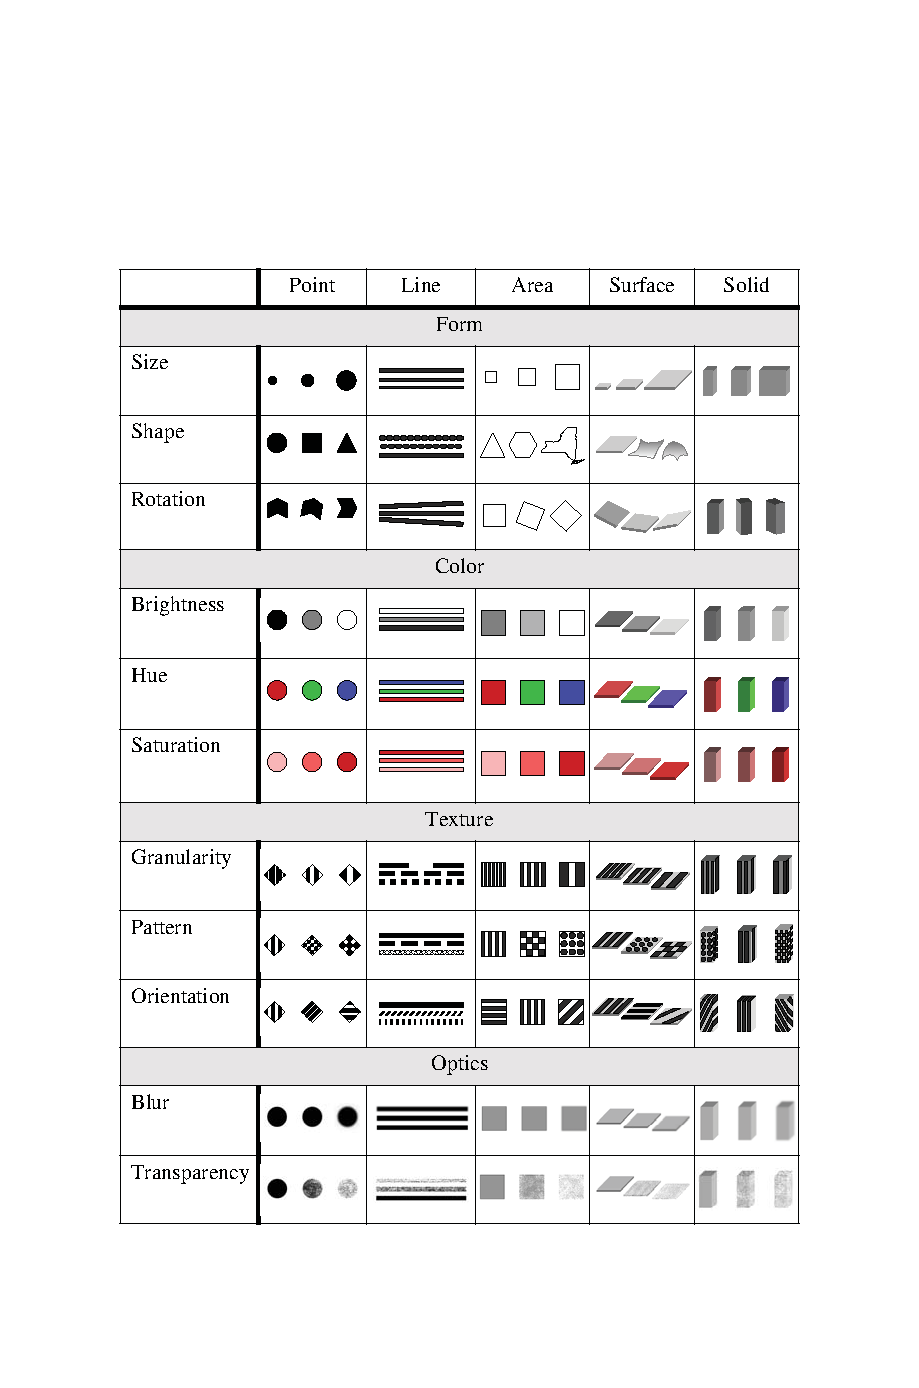
\includegraphics[width=0.8\textwidth]{figures/aesthetic_attributes.pdf}
    \caption{Aesthetic Attributes by Geometry~\cite{Wilkinson05grammar}.}
    \label{fig:aesthetic-attributes}
  \end{center}
\end{figure}

Information on a map is represented by symbols, point, lines or areas with properties such as color and shape. Bertin~\cite{bertin67graphics, bertin83graphics} has described the fundamental graphic variables for map and graphic design. While being written for hand-drawn maps on paper, the concepts described by Bertin are still applied in todays digital mapping applications and have been further developed by MacEachren~\cite{MacEachren95maps}.

The main variables, introduced by Bertin are: \textit{location}, \textit{size}, \textit{value}, \textit{texture}, \textit{color}, \textit{orientation} and \textit{shape}. MacEachren adds \textit{crispness}, \textit{resolution}, \textit{transparency} and \textit{arrangement} to the list and splits up color into its values of \textit{brightness}, \textit{saturation} and \textit{hue}. Figure \ref{fig:aesthetic-attributes} describes a similar list of aesthetic attributes by different geometries and groups the variables regarding \textit{form}, \textit{color}, \textit{texture} and \textit{optics}~\cite{Wilkinson05grammar}.

Each variable has a different potential for visualizing data of categorical information (nominal and ordinal) or numerical information (including intervals and ratios). For example, the size of a point can be used to describe a numeric ratio and different shapes may be used to distinguish items based on categories. On the other hand, different texture patterns only offer a limited set of possibilities and size shouldn't be used for describing nominal properties~\cite{noellenburg11geovis, MacEachren95maps}. 

\section{Visual data exploration techniques}
\label{vis-data-techniques}

Depending on the task and the type of data to be shown, different forms of visualization and techniques for exploring the data exist. Daniel A. Keim~\cite{keim2001vis} classifies such techniques using three criteria as depicted in figure \ref{fig:visual-techniques}: the \textit{data type} to be visualized, the \textit{technique} itself and the \textit{interaction and distortion} method~\cite{Delort10vis}:

\begin{itemize}

\item The \textbf{data type} is classified into \textit{one-dimensional} (as for example temporal data), \textit{two-dimensional} (geographical maps), \textit{multi-dimensional} (relational tables), \textit{text and hypertext} (articles and web documents), \textit{hierarchies and graphs} (networks) as well as \textit{algorithms and software} (such as debugging operations).

\item The \textbf{visualization techniques} are classified into \textit{standard 2d/3d displays} (x-y plots and landscapes), \textit{geometrically-transformed displays} (parallel coordinates), \textit{iconic displays} (glyphs), \textit{dense pixel displays} (recursive pattern) and \textit{stacked displays} (tree maps).

\item Finally, the third dimension describes the \textbf{interaction technique} being used, such as \textit{dynamic projection}, \textit{interactive filtering}, \textit{zooming}, \textit{distortion} and finally \textit{link \& brush} approaches.

\end{itemize}

\begin{figure}[h]
  \begin{center}
    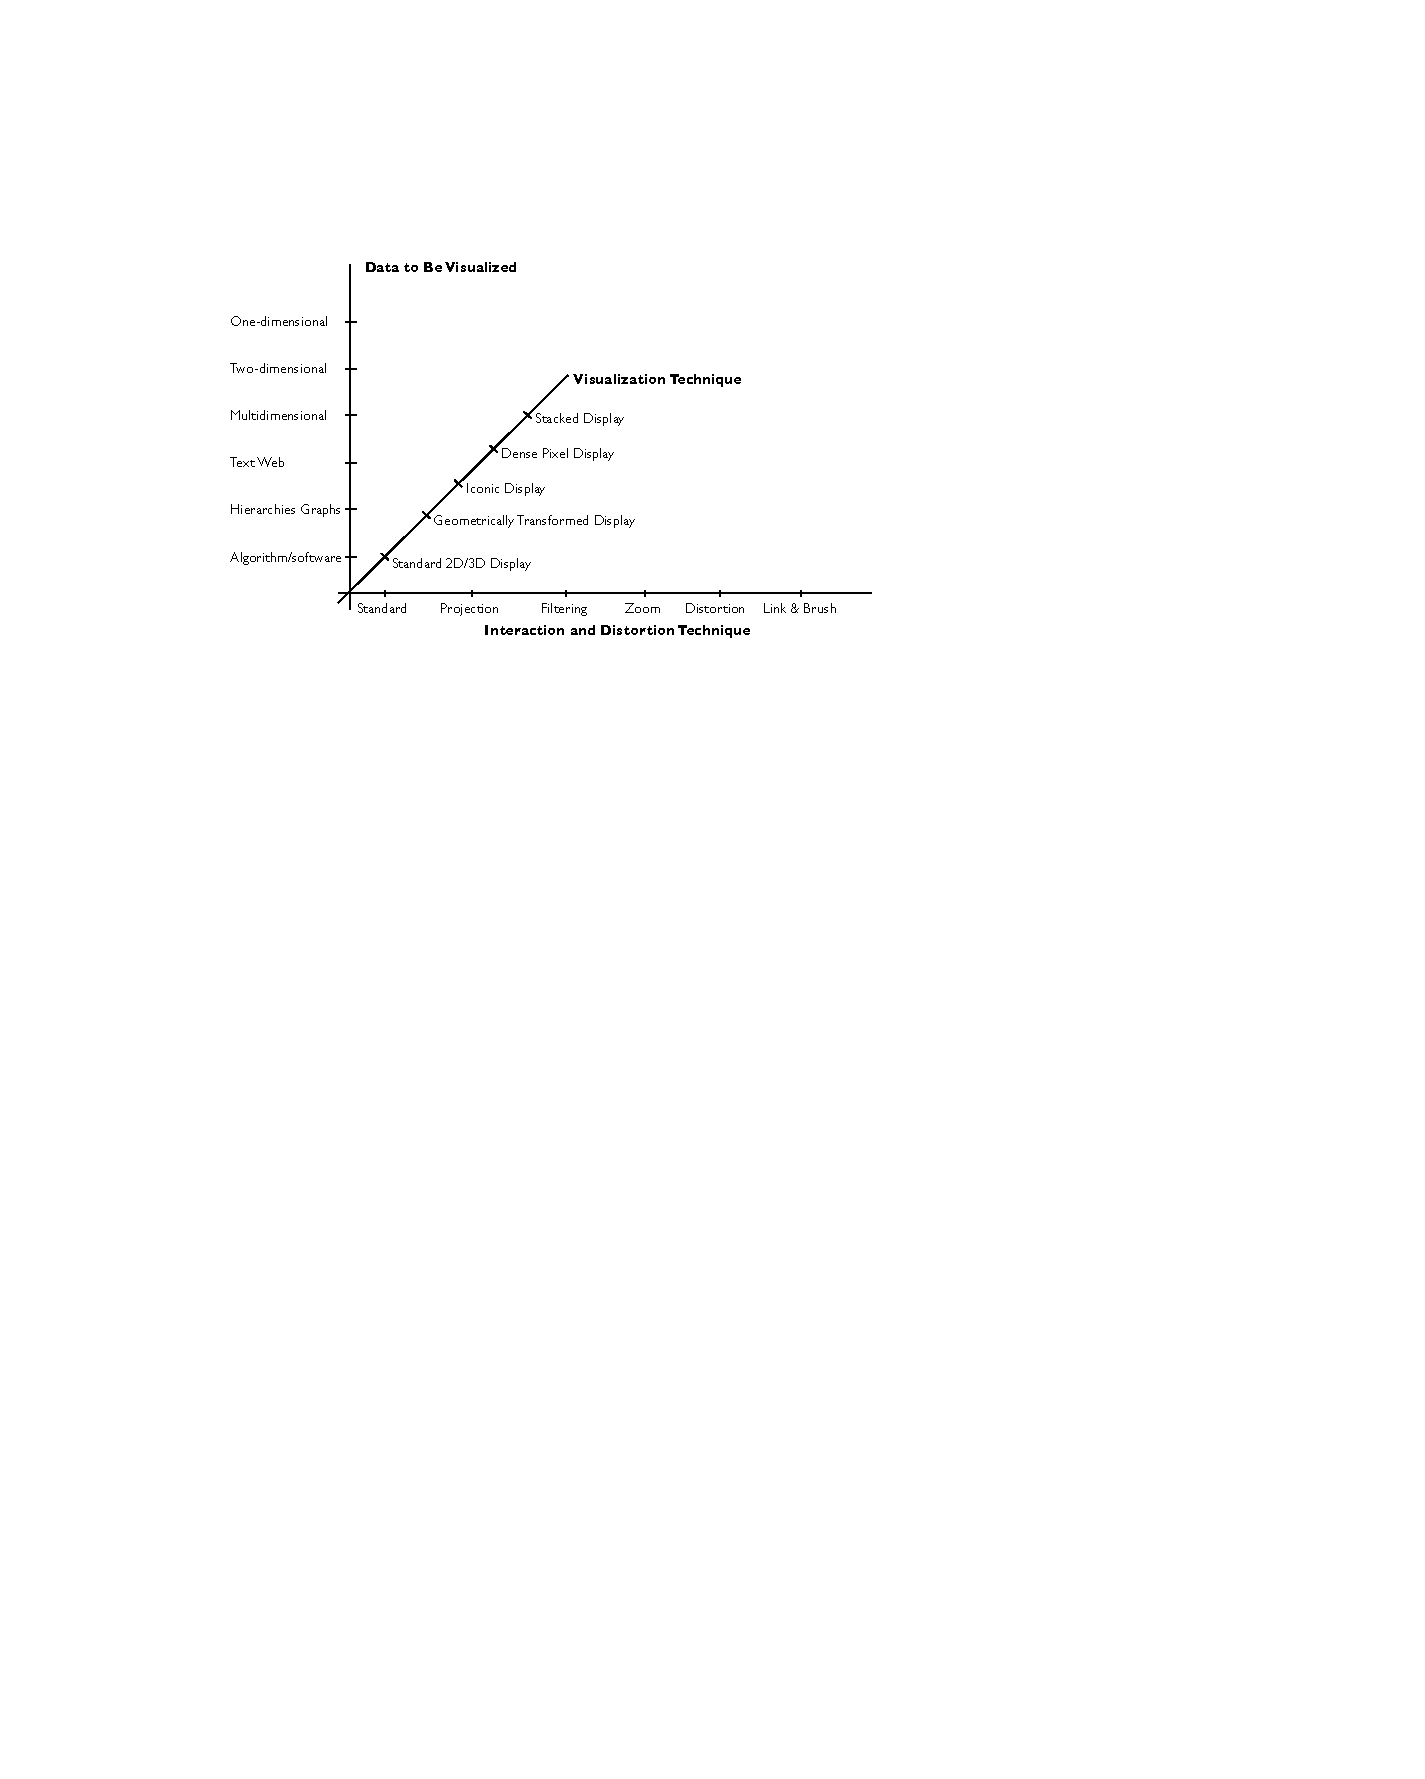
\includegraphics[width=1\textwidth]{figures/classes_visual_techniques.pdf}
    \caption{Classification of visual data exploration techniques based on~\cite{keim2001vis}.}
    \label{fig:visual-techniques}
  \end{center}
\end{figure}


With regards to visualizing clusters on a map, it appears that the visualization technique may be considered from two different view points:

\begin{itemize}

\item the visualization of the \textit{entire map} with clustered points on it, as well as

\item the visualization of an \textit{individual cluster}, placed on the map.

\end{itemize}

A typical map for representing spatially clustered data is based on a least \textit{two-dimensional data}, containing latitude and longitude information of cluster items. The map is presented in planar space, which classifies it amongst \textit{standard 2d/3d displays}. Common interaction techniques for maps are \textit{zooming} and \textit{panning} which allow the user to explore the 2-dimensional space and reveal details.

The visualization of individual clusters on the map is likely to be classified amongst \textit{iconic displays}. During the clustering process, individual points get aggregated, which potentially leads to multivariate aggregate information of item properties. Depending on the level of detail that clusters should expose, more complex visualization techniques may be possible. 

Approaches for visualization techniques of the entire map and individual clusters will be discussed further in chapter  \ref{state-vis}.

\section{Clutter reduction}
\label{clutter-reduction}

Clutter reduction is a way to enhance readability and general performance of maps. An early publication about \textit{visual clutter} on maps by Richard J. Phillips and Liza Noyes~\cite{phillips82clutter} states that ``reducing visual clutter improves map reading performance''. Clutter reduces the background visibility and prevents the user from understanding structure and content of the data being presented. This especially becomes true for visualizing large data sets on maps, so that properties of the data items are hardly visible~\cite{harvey2008primer, Delort10vis}.

Clustering of course is the approach for clutter reduction that is primarily being investigated for this thesis. In order to review the effectiveness and limitations of clustering, as well as the relationship that it has to other techniques in that field, it is helpful to review the ``Clutter Reduction Taxonomy'' by Geoffrey Ellis and Alan Dix~\cite{ellis08clutter}. It distinguishes between three main types of clutter reduction techniques:

\begin{itemize}

\item \textbf{appearance}: alter the look of data items by using techniques like \textit{sampling}, \textit{filtering}, \textit{changing point sizes}, \textit{changing opacity} or \textit{clustering}.

\item \textbf{spatial distortion}: displace the data items in ways as \textit{point/line displacement}, \textit{topological distortion}, \textit{space-filling}, \textit{pixel-plotting} or \textit{dimensional reordering}.

\item \textbf{temporal}: use \textit{animation} to reveal additional information.

\end{itemize}

In a next step, the stated techniques have been evaluated against a list of 8 high-level criteria~\cite{ellis08clutter}. For this thesis, the relevant information for the clustering technique have been extracted and will be outlined by each criterium:

\begin{enumerate}

\item \textit{avoids overlap}
\\ The major benefit is to reduce clutter, provide the ability of seeing and identifying patterns, have less hidden data, as well as giving more display space to points. Clustering can be used in such a way to avoid \textit{overplotting} by representing groups of points as single points.

\item \textit{keeps spatial information}
\\ Maintaining the correct coordinates of items is relevant, but the study also states that relative positions of points might have greater influence on orientation than just their exact coordinates. Clustering by definition looses the spatial information of individual points, but using aggregate values, like the centroid a cluster, as the position can be used for compensation. 

\item \textit{can be localized}
\\ The term localization is used to specify, if the display can be reduced to a specific region. This is usually provided by \textit{focus and context} techniques that reveal information underneath by zooming into an area. The study doesn't make a clear decision regarding the applicability of localization for clustering and states that different properties for spatial and non-spatial clustering apply. In the case of spatial clustering, localization is definitely possible and has been implemented, see chapter \ref{chapter:realization}.  

\item \textit{is scalable}
\\ Scalability of the clutter reduction technique with regards to large amounts of data is the goal of this criterium. The study admits that the meaning of large datasets is vaguely quantified. As one of the main goals for this thesis is to enhance performance for large data sets by using clustering, the technique is expected to satisfy this condition. Of course, the range of scalability depends on the implemented clustering algorithm. Also refer to the time complexity definitions in chapter \ref{clustering-algorithms}. 

\item \textit{is adjustable}
\\ If the user is able to control aspects of the visual display and adjust parameters of the system that influence the degree of display clutter. Scientific methods in cluster analysis tend to offer a a higher level of interactivity, while public facing clustering applications limit the amount of interactivity to controlling cluster sizes and the previously discussed localizing feature. 

\item \textit{can show point/line attribute}
\\ The goal is to map attributes of the data to properties like color, shape or opacity of the displayed points or lines. For clustering, this feature can be used in order to display aggregates of the multivariate data results from the clustering process. Further information can be found in chapter \ref{chapter:cluster-vis}.

\item \textit{can discriminate points/lines}
\\ Being to able to identify individual data items within a crowded display is the goal of this criterium. The study states the capability of clustering for detecting outliers as well as creating groups of points in order to satisfy this criterion. On the other hand, this classification appears unclear, as the grouping process of clustering aggregates individual information by definition and only makes it accessible by request or localization. 

\item \textit{can see overlap density}
\\ This helps to gauge the amount of overplotting, see where higher density regions are and understand the distribution of data underlying the visualization. Clustering can show the amount of items within clusters by using visual indicators as point size, opacity and color.  

\end{enumerate}



%
% state - vis
%

\chapter{Results}
\label{state-vis}

In the previous chapter, foundations of visualization, visual variables and data exploration techniques, as well as the concept of clutter reduction have been introduced. As the main part of the presented study, existing visualization techniques for representing clustered data on maps will be discussed. In a first step, visualization concepts on the map level will be investigated. Later, approaches for visualizing individual clusters are added. An evaluation summarizes the discussed technologies.

\section{Map visualization types for clustering}
\label{chapter:map-vis}

There exists a variety of map types, serving different purposes like standard \textit{geographic maps}, \textit{cartograms}, \textit{geologic maps}, \textit{linguistic maps} or \textit{weather maps}. Some of these use distortion, for example the cartogram can be used to map the area of each country to the size of population. In this section, we try to identify those map types which are appropriate for visualizing clustered data~\cite{noellenburg11geovis, wiki:map-types}:

\begin{itemize}

\item \textbf{Geographic map with markers}. The default way of representing data is a standard 2-dimensional map with markers on top of it. Each marker represents a data point, or in the case of clustering, a cluster.

\parbox [h]{0.4\textwidth}{
    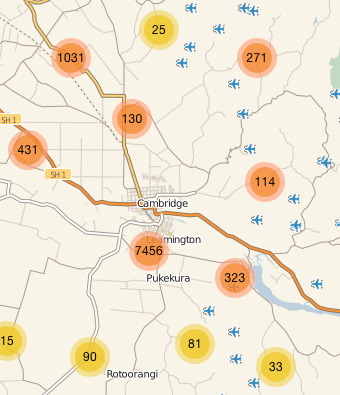
\includegraphics [width=\linewidth]{figures/map_types_normal_leaflet.png}
    \captionof {figure}{Leaflet map}
    \label{fig:map-type-standard-leaflet}
}
\hfill
\hspace{0.5cm}
\parbox [h]{0.4\textwidth }{
    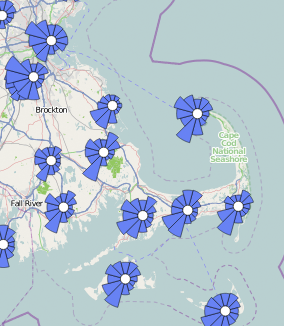
\includegraphics [width=\linewidth]{figures/map_types_standard_wind.png}
    \captionof {figure}{Wind history map}
    \label{fig:map-type-standard-wind}
}

\begin{itemize}

\item Figure \ref{fig:map-type-standard-leaflet} depicts an example\footnote{Leaflet.clustermarker example map from \url{http://leaflet.github.io/Leaflet.markercluster/example/marker-clustering-realworld.10000.html}} of the Leaflet.markercluster library. Clustered results are displayed using markers of the same size. The amount of items within a cluster is indicated using text within the markers and by using a ``hot-to-cold'' color ramp~\cite{web:color-ramp}. 

\item Figure \ref{fig:map-type-standard-wind} shows a similar example, in this case a Wind history map\footnote{Wind history map \url{http://windhistory.com/map.html}} with markers for every wind measurement point. An advanced visualization technique is used for visualizing the amount of wind per cardinal direction as \textit{polar area diagram}.

\end {itemize}

These two variations of standard maps shall indicate the potential of using advanced visualization techniques for displaying cluster items. Further ways for cluster visualization will be discussed in chapter \ref{chapter:cluster-vis}.

\item \textbf{Geographic Heat map}

Heat maps use colored, two-dimensional areas to express the value of each data entity on the map. \textit{Choropleth maps} are the most common heat maps, which are often used for analysis of geographic and statistical data. 

\parbox [h]{0.4\textwidth}{
    
\includegraphics [width=\linewidth]{figures/map_types_choropleth.pdf}
    \captionof {figure}{Choropleth map\protect\footnotemark}
    \label{fig:map-type-choropleth}
}\footnotetext{Choropleth map example from Kartograph \url{http://kartograph.org/showcase/choropleth/}}
\hfill
\hspace{0.5cm}
\parbox [h]{0.4\textwidth}{
    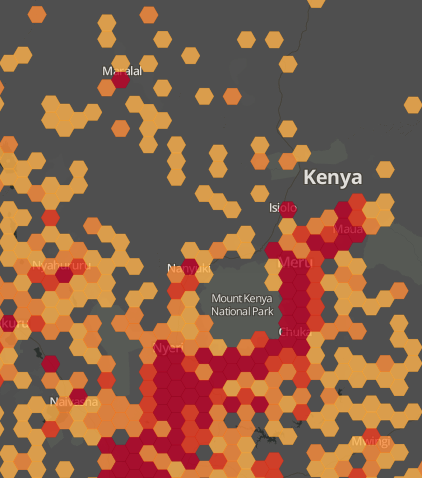
\includegraphics [width=\linewidth]{figures/map_types_heatmap.png}
    \captionof {figure}{Heat map\protect\footnotemark}
    \label{fig:map-type-binning}
}\footnotetext{Heat map that uses binning \url{http://mapbox.com/blog/binning-alternative-point-maps/}}


\begin{itemize}

\item Figure \ref{fig:map-type-choropleth} visualizes an example choropleth map that shows population data for each of the departments of metropolean France. Color coding is used to indicate densely populated regions with heavier red tones.

\item Figure \ref{fig:map-type-binning} presents another example that uses \textit{binning} for creating a hexagonal tessellation of the surface in order to visualize clustered results. 

\end {itemize}

A problem with heat maps is that they require a non-overlapping tessellation of the surface to provide the areas for visualization. As the binning example indicates, such a tessellation can be done programmatically. Heat maps therefore can also be used for visualizating arbitrary clustered data without a need to calculate the exact boundaries of clusters. Another variation of heat maps is the \textit{prism map}, which adds extrusion of areas as a third dimension~\cite{ladenhauf12dia, Delort10vis}. A publication on the evaluation of color schemes in choropleth maps can be found in~\cite{MacEachrenMort}. 


\item \textbf{Dot grid maps}

Dot grid maps are based on the suggestion by Jaques Bertin~\cite{bertin67graphics, bertin83graphics} to use graduated sizes in a regular pattern as an alternative to chloropeth maps. The advantage is that the map creator doesn't have to choose between quantity or density of a distribution value, because the dot grid map shows both a the same time. The user can understand the data distribution on a finer level of granularity, as opposed to where the chloropeth map usually creates larger areas of aggregated information~\cite{web:dot-grid}.

Figure \ref{fig:map-type-dotgrid} is an alternative version of the France map from figure \ref{fig:map-type-choropleth}, visualized as a dot grid map.


\item \textbf{Voronoi map}

The Voronoi tessellation is a space partitioning technique. From a set of points it produces a Voronoi polygon for each point, such that the area covered is closest to that point in comparison to all other points. Jean-Yves Delort describes a technique that uses Voronoi polygons for ``Vizualizing Large Spatial Datasets in Interactive Maps''~\cite{Delort10vis}. It uses a hierarchical clustering technique to choose a subset of points per zoom level for proper visualization. Still, the effectiveness of this approach is questionable, as the scalability analysis of the studies shows that the technique can efficiently be used for datasets of up to 1000 items.

Figure \ref{fig:map-type-voronoi} shows an exemplary voronoi map that displays all U.S. airports as of 2008. Besides the shown visualization, for Voronoi maps apply the same visualization possibilities as for cloropeth maps.

\parbox [h]{0.4\textwidth }{
    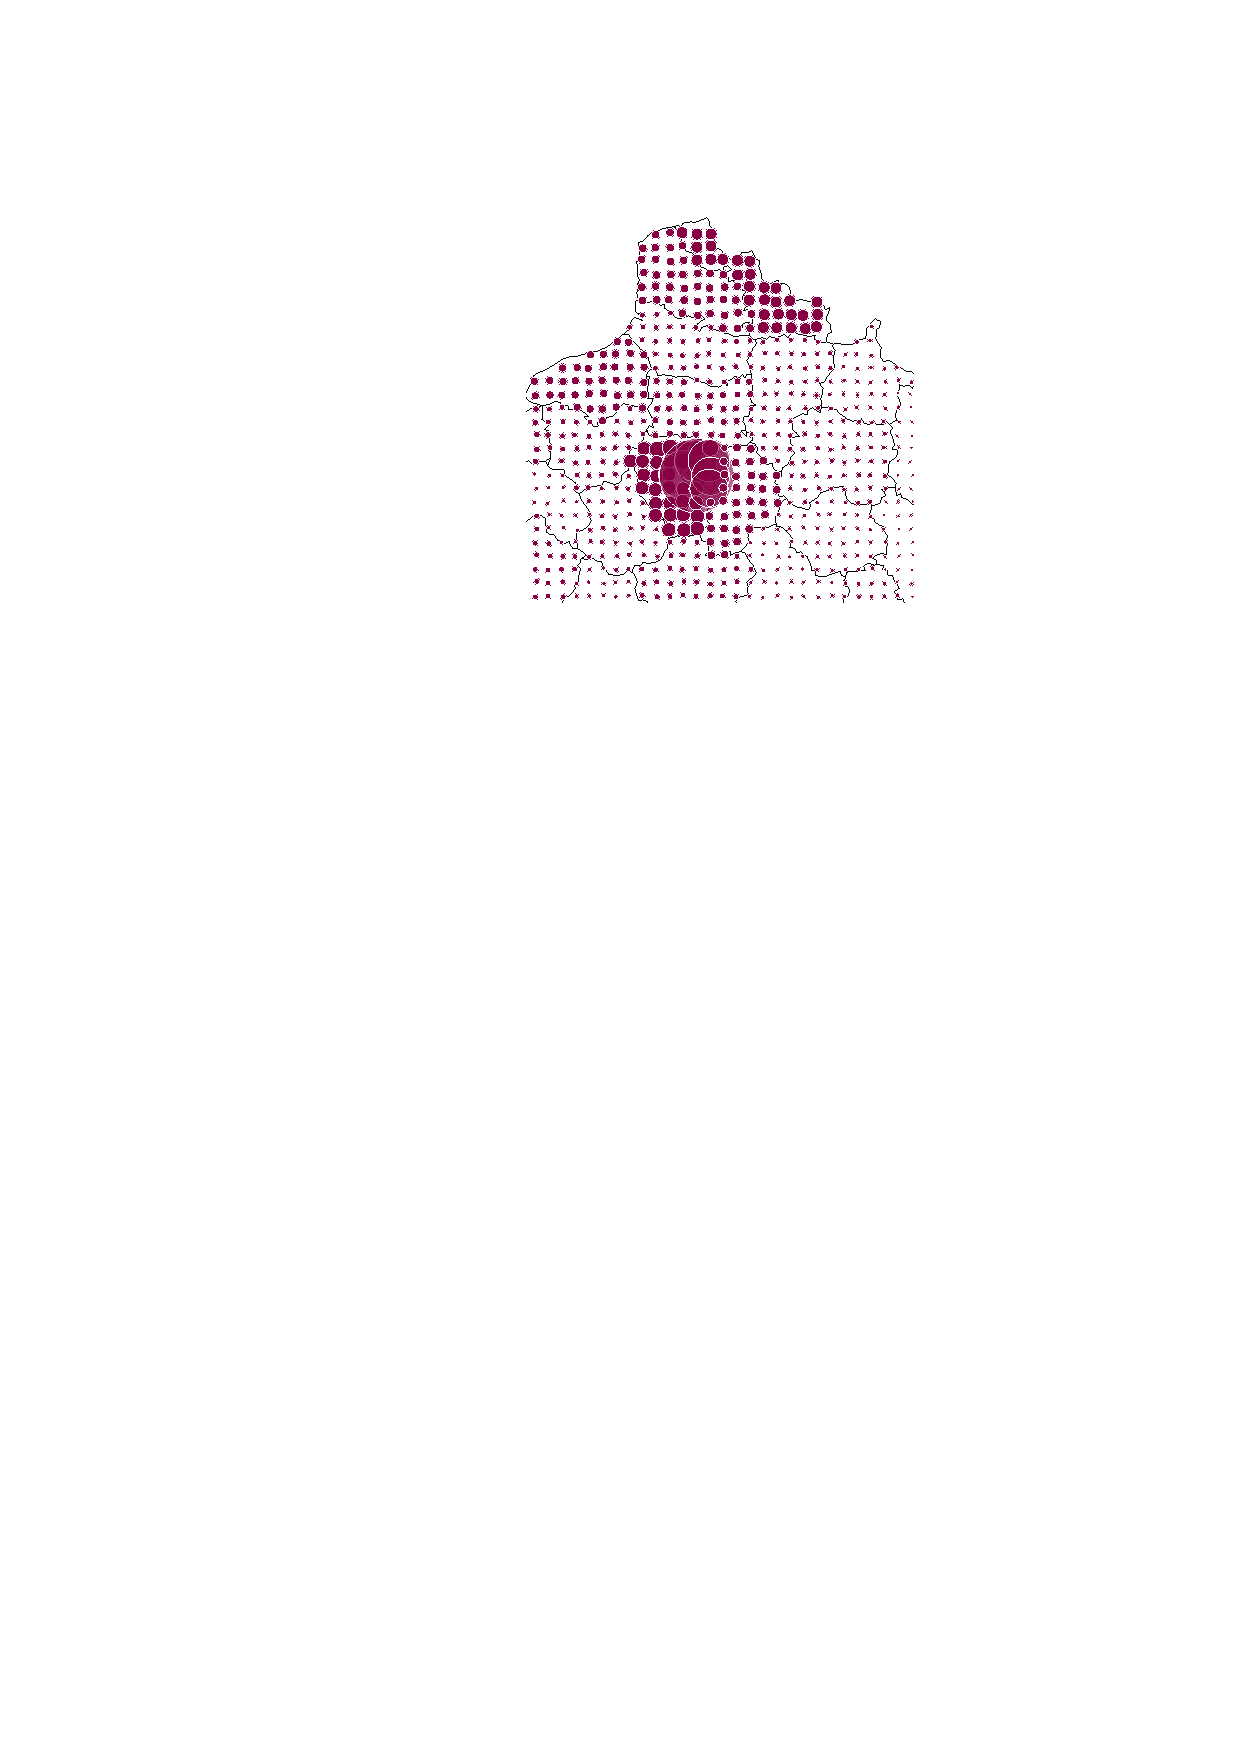
\includegraphics [width=\linewidth]{figures/map_types_dot_grid.pdf}
    \captionof {figure}{Dot Grid map\protect\footnotemark}
    \label{fig:map-type-dotgrid}
}\footnotetext{Dot Grid map example from Kartograph \url{http://kartograph.org/showcase/dotgrid/}}
\hfill
\hspace{0.5cm}
\parbox [h]{0.4\textwidth }{
    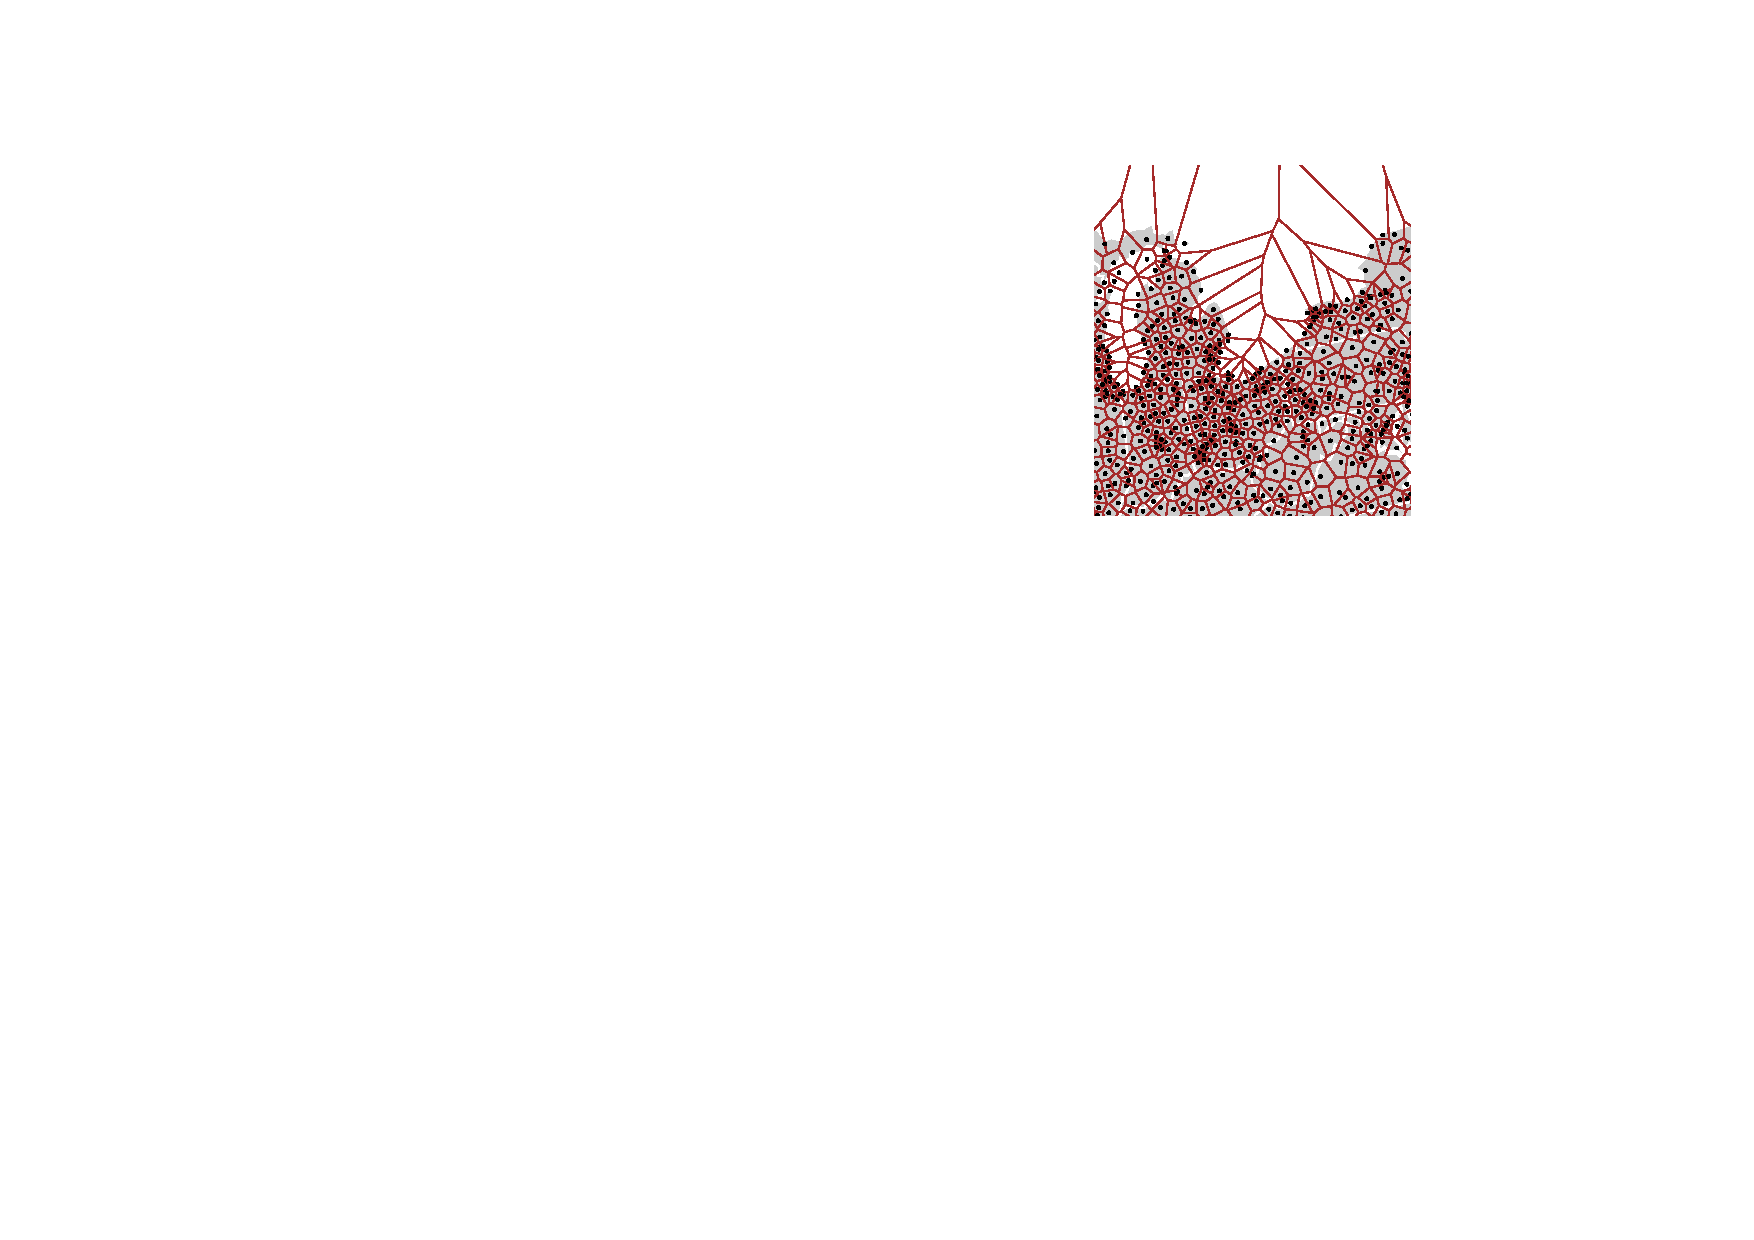
\includegraphics [width=\linewidth]{figures/map_types_voronoi.pdf}
    \captionof {figure}{Voronoi map\protect\footnotemark}
    \label{fig:map-type-voronoi}
}\footnotetext{Voronoi map example \url{http://mbostock.github.io/d3/talk/20111116/airports-all.html}}

\end{itemize}

\textit{Self-organizing maps} (SOM) can also be used to visualize clusters of data. But instead of displaying data on a geographic map, self-organizing maps create their own virtual space in order to represent information~\cite{noellenburg11geovis}.  


\section{Cluster visualization techniques for maps}
\label{chapter:cluster-vis}

The previous chapter has shown different kinds of map visualization techniques appropriate for displaying clustered data. In the end, each visualization will show (clustered) items on a map as visual objects with attributes like a particular shape or coloring. As clusters contain aggregated information, an important task is to find the right way for visualizing the cluster items themselves. From the examples provided so far, we have seen variations in size, shape and color which expose information on the cluster items being visualized on the map. In the following, multivariate data visualization techniques will be evaluated for visualizing cluster items on a map.

In chapter \ref{vis-data-techniques}, a classification of visualization techniques by data type and interaction technique has been presented. Ke-Bing Zhang~\cite{zhang07thesis} has written about ``Visual Cluster Analysis in Data Mining'', where he list an extensive list of multivariate data visualization techniques. Potentially, any such visualization technique can be used, but the frame of the map puts constraints in terms of space on the representation of individual items. \textit{Iconic displays} are a simple way to visualize data, which also prevents clutter. \textit{Dense Pixel} displays and \textit{geometric visualizations} like charts can be used to encode more complex information.

\begin{itemize}

\item \textbf{Icon-based, Glyphs}

Matthew O Ward \cite{ward02glyphs} defines \textit{glyphs} as ``graphical entities that convey one or more data values via attributes such as shape, size, color, and position''. While the work of Otto Neurath on \textit{ISOTYPE}~\cite{neurath} (1930s) can be seen as fundamental for \textit{pictorial statistics}, the best-known literature reference to glyphs is ``Chernoff faces''~\cite{chernoff73}. As (e) figure \ref{fig:glyphs-ward} indicates, data is encoded into properties of the face icon, such as shape of nose, mouth, eyes. Other fundamental glyph-based techniques include \textit{stick figures}~\cite{stickfigures}, \textit{color icons}~\cite{coloricons}, \textit{Hyperbox}~\cite{hyperbox} and \textit{shape coding}~\cite{shapecoding}. Figure \ref{fig:glyphs-ward} extends this list by showing examples of glyphs that Ward collected for his taxonomy of glyphs placement strategies~\cite{ward02glyphs}.

\begin{figure}[h]
  \begin{center}
    \hspace*{-1cm}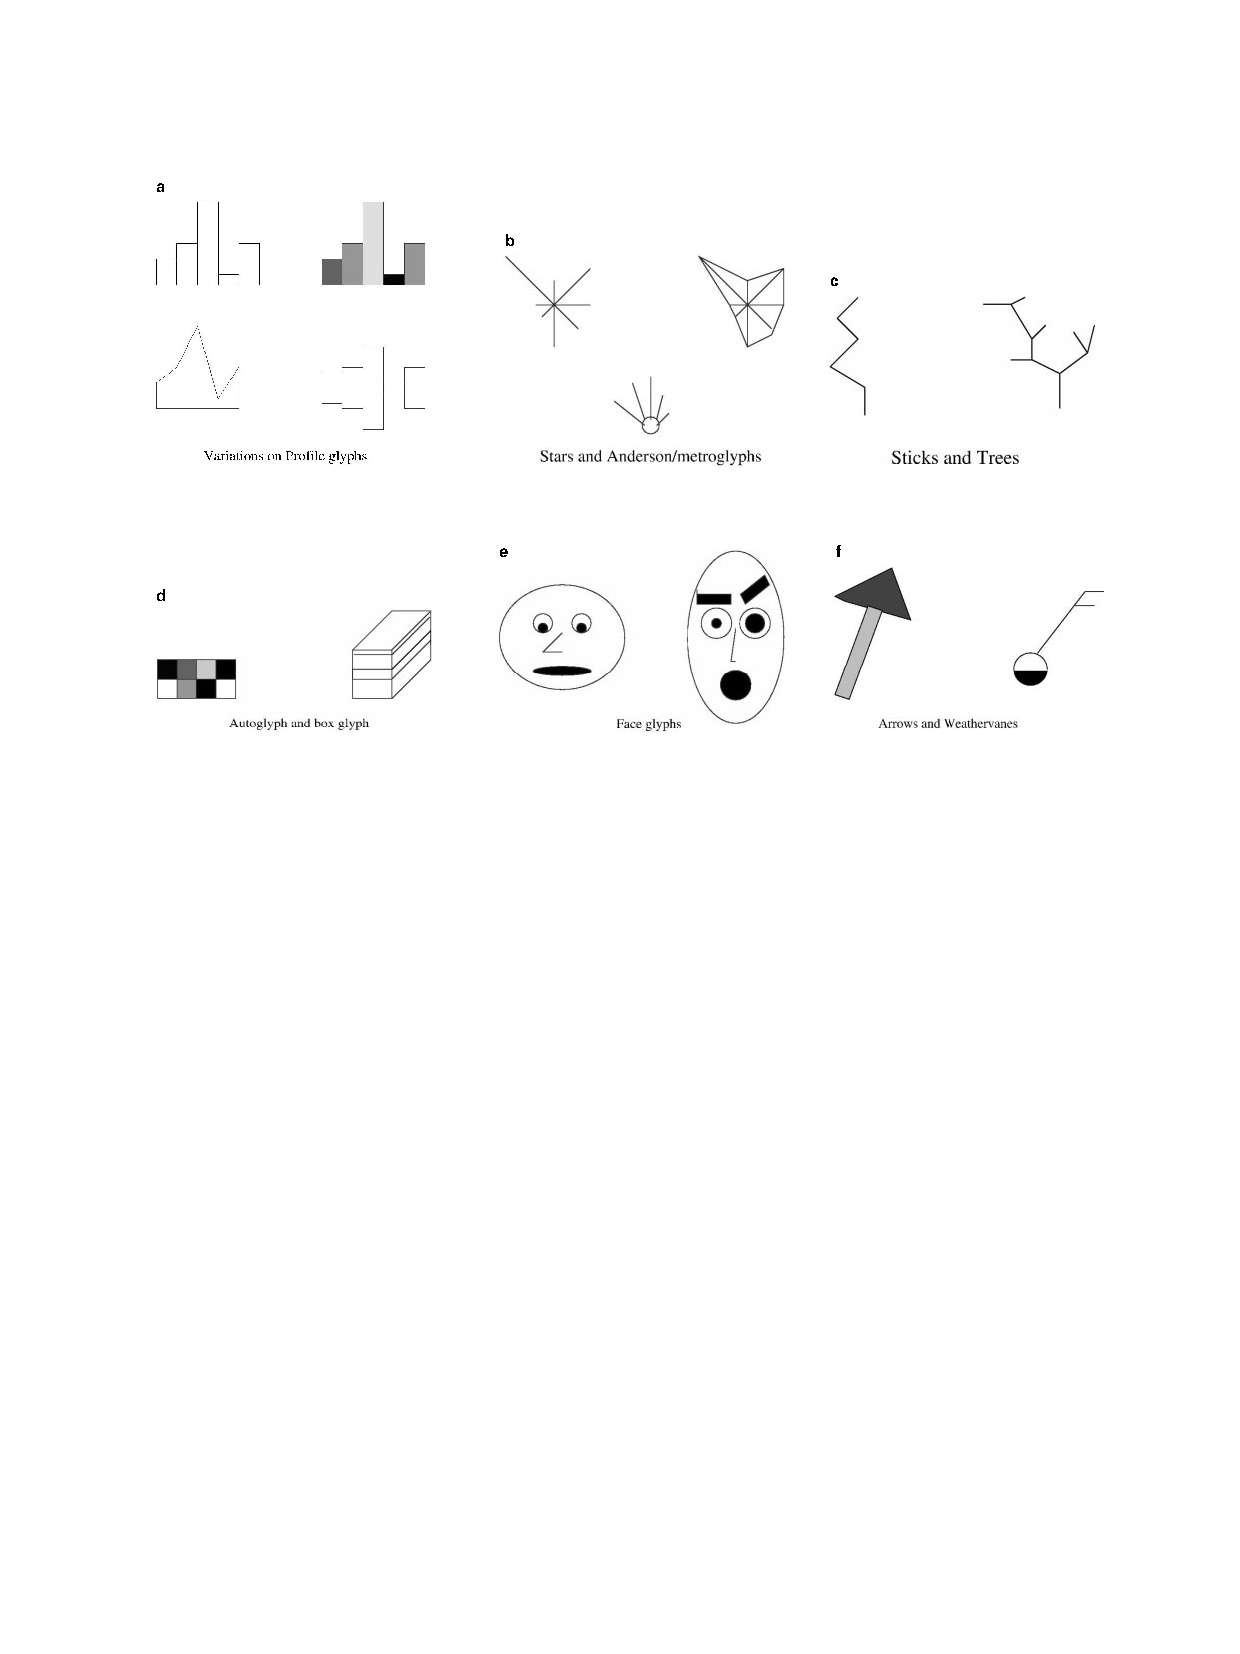
\includegraphics[width=1.2\textwidth]{figures/glyphs.pdf}
    \caption{Examples of glyphs. Top row: (a) variations on profiles; (b) stars/metroglyphs; and (c) stick figures and trees.
Bottom row: (d) autoglyphs and boxes; (e) faces; and (f) arrows and weathervanes.~\cite{ward02glyphs}.}
    \label{fig:glyphs-ward}
  \end{center}
\end{figure}

Some glyph types have been created to identify clusters or similarities by plotting them side-by-side on a 2-dimensional plane, a technique which is referred to as \textit{mosaic-based rendering}. \textit{Stick figures} and \textit{mosaic metaphors} are examples in that field~\cite{stickfigures, nocke05mosaic}. One the other hand, reducing visual clutter as explained in chapter \ref{clutter-reduction} also matters for glyphs, especially when putting them on a map. A trade-off between information-richness vs. simplicity and clarity has to be made. As Zhang writes, ``with the amount of data increasing, the user hardly makes any sense of most properties of data intuitively, this is because the user cannot focus on the details of each icon when the data scale is very large''~\cite{zhang07thesis}. We can compare this to the map use cube presented in chapter \ref{chapter:foundations-vis}: more complex glyph types seem to be better suited for scientific purposes which can be related to private uses, while simpler glyph types seem more appropriate for presenting data to a public audience.

Examples for uses of simple icons and glyph types for clustered data on maps can be found in JavaScript mapping libraries like Leaflet. These are usually based on a simple icon or geometric shape like a circle or marker and use color coding and size variations as indicators for underlying information. Further examples are scaled data values and scaled dots \cite{web:scaled-data-value}, as well as the proportional symbol map \cite{vislecture}. In contrast to those presented so far, figure \ref{fig:glyphs-zame} visualizes eight simple glyphs~\cite{ElmqvistDGHF08}.

\begin{figure}[h]
  \begin{center}
    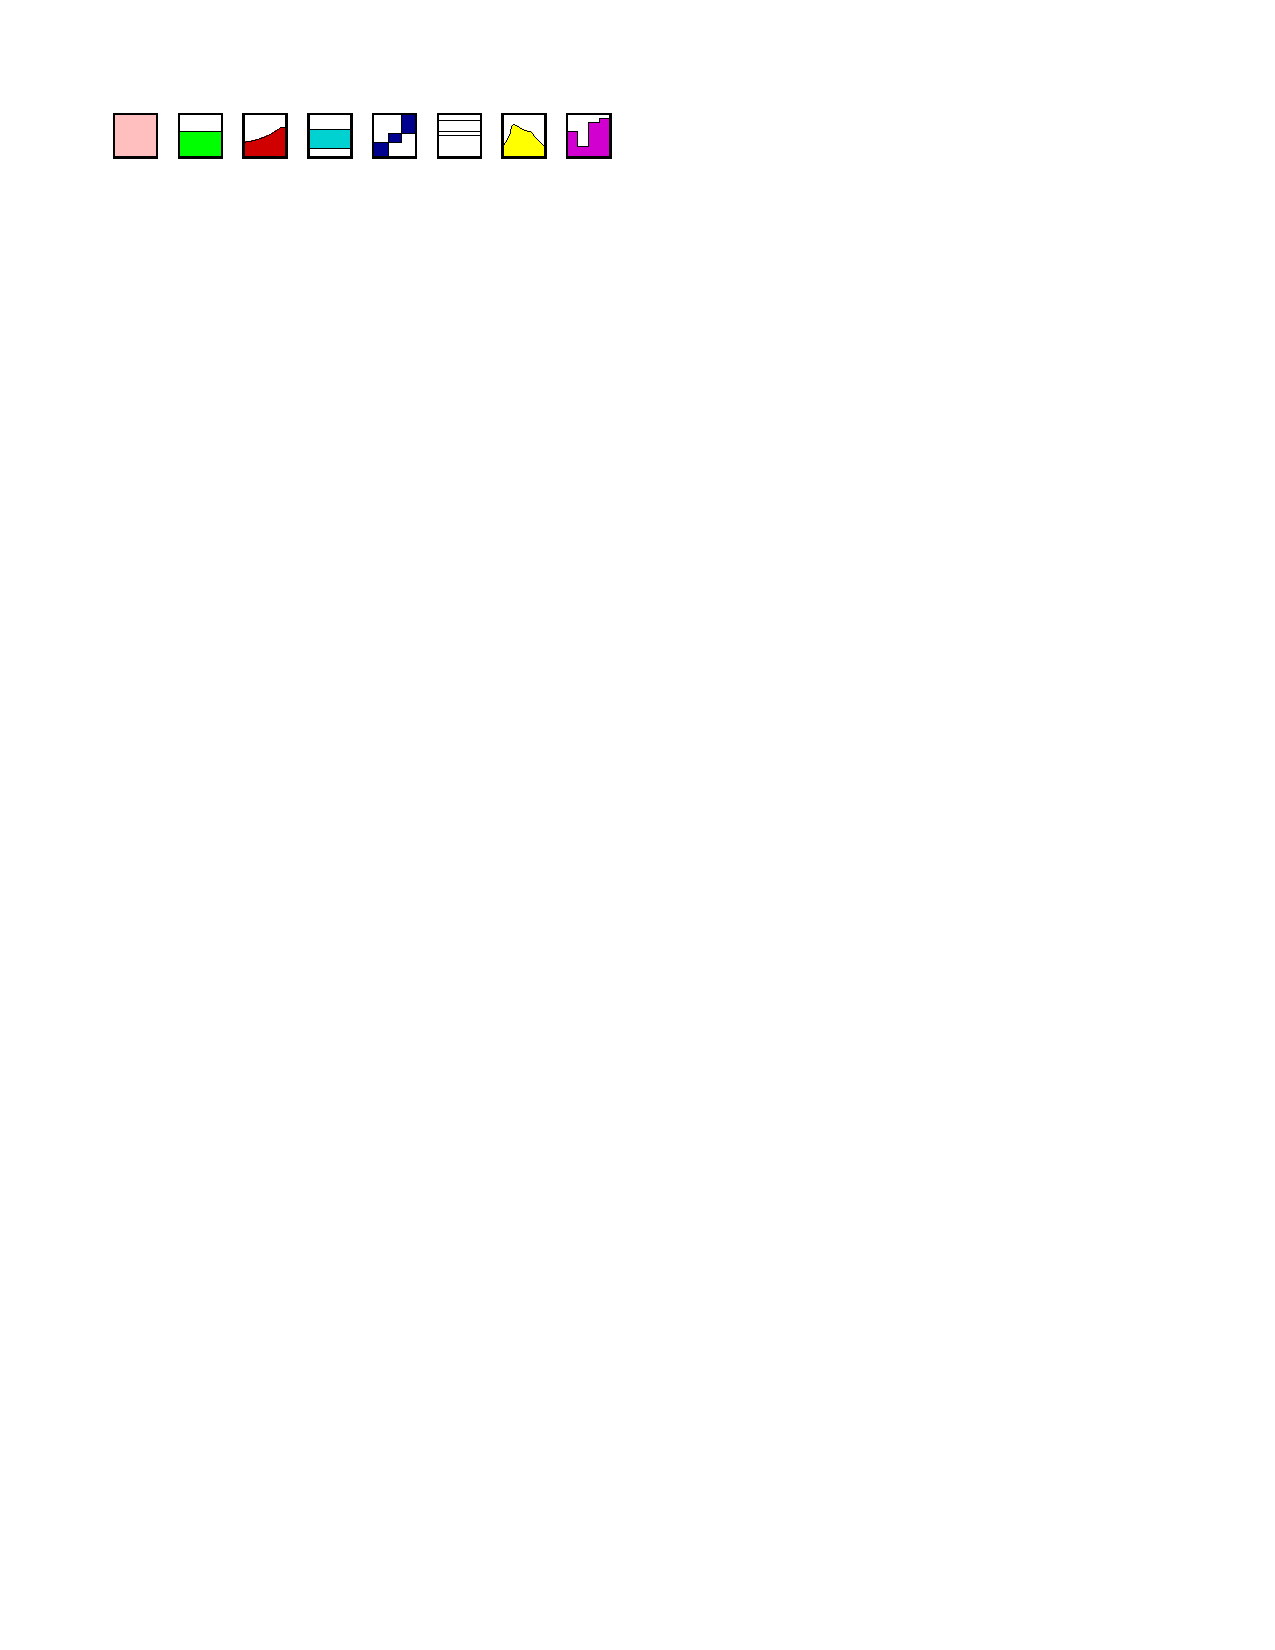
\includegraphics[width=0.65\textwidth]{figures/glyphs_zame.pdf}
    \caption{Eight different glyphs for aggregated edges (color shade,
average, min/max histogram, min/max range, min/max tribox, Tukey
box, smooth histogram, step histogram)~\cite{ElmqvistDGHF08}.}
    \label{fig:glyphs-zame}
  \end{center}
\end{figure}


\item \textbf{Pixel-oriented}

Pixel-oriented techniques display the most possible information at a time by mapping each attribute value of data to a single, colored pixel. Color mapping approaches such as \textit{linear variation of brightness}, \textit{maximum variation of hue} and \textit{constant maximum saturation} are used to color pixels which are arranged within limited space. By providing an overview of large amounts of data, pixel-oriented display techniques are suitable for a variety of data mining tasks in combination with large databases~\cite{zhang07thesis}.

The first pixel-oriented technique was presented by Keim~\cite{keim94pixel} as part of the \textit{VisDB system}. Large amounts of multidimensional data are represented as \textit{Spirals} and \textit{Axes}. Figure \ref{fig:pixel-spiral} illustrates how a spiral would be constructed and figure \ref{fig:pixel-axes} shows a rendered result of the axes technique. Further developments include the \textit{Recursive Pattern Technique} \cite{keim95recpat} and the \textit{Circle Segments Technique} \cite{Ankerst96circlesegments}. Figure \ref{fig:pixel-circle} visualizes such a circle which represents about 265,000 50-dimensional data items.

While no real-world examples have been identified during the research, using pixel-oriented techniques for visualizing complex clusters on a map seems possible. As the visualization relies on a large amounts of multidimensional data being present within clusters, the clustering algorithm would need to provide such required data. Performance implications also have to be considered, as potentially multiple clusters will be visualized on a map, sometimes even in real-time.

\hspace*{-2cm}\parbox [h]{0.35\textwidth }{
    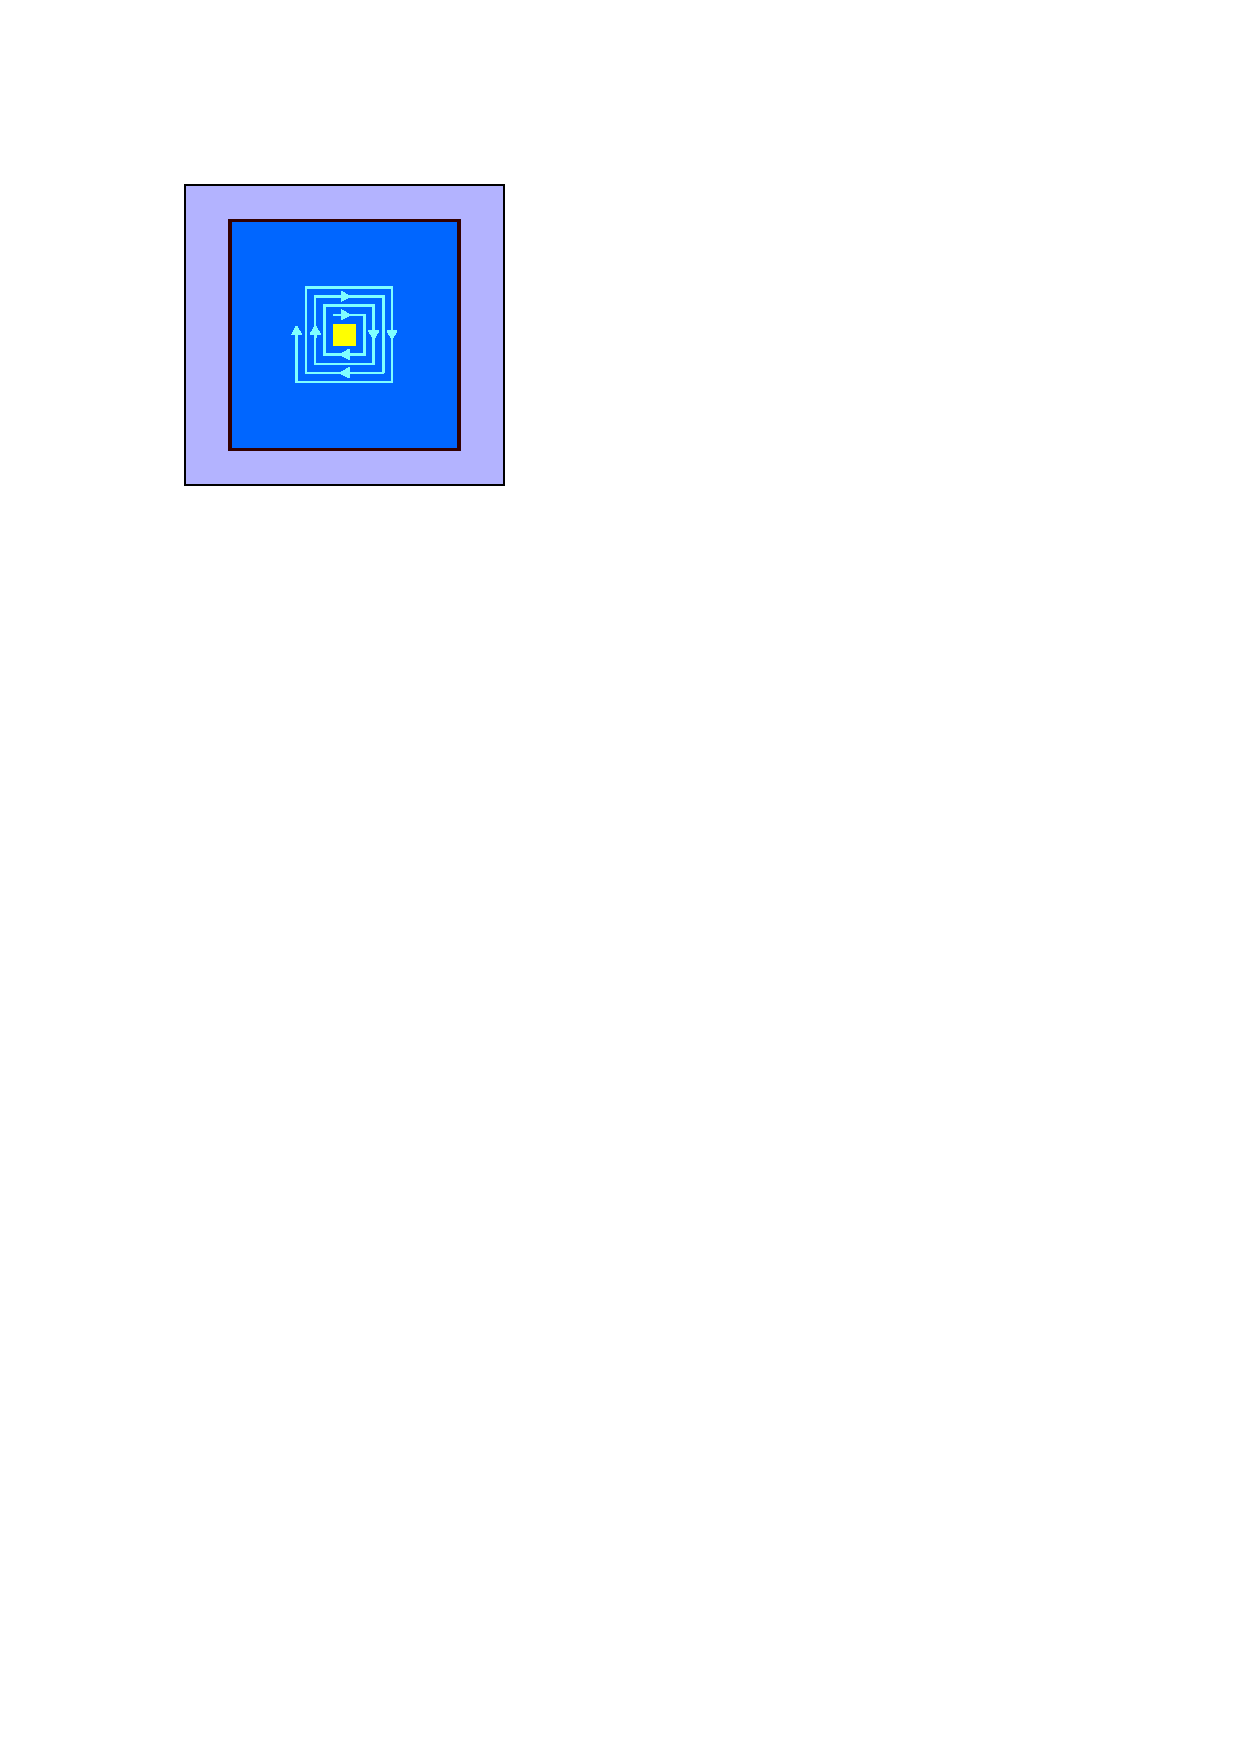
\includegraphics [width=\linewidth]{figures/pixel_keim_spiral.pdf}
    \captionof {figure}{Spiral~\cite{keim94pixel}}
    \label{fig:pixel-spiral}
}
\hfill
\parbox [h]{0.33\textwidth }{
    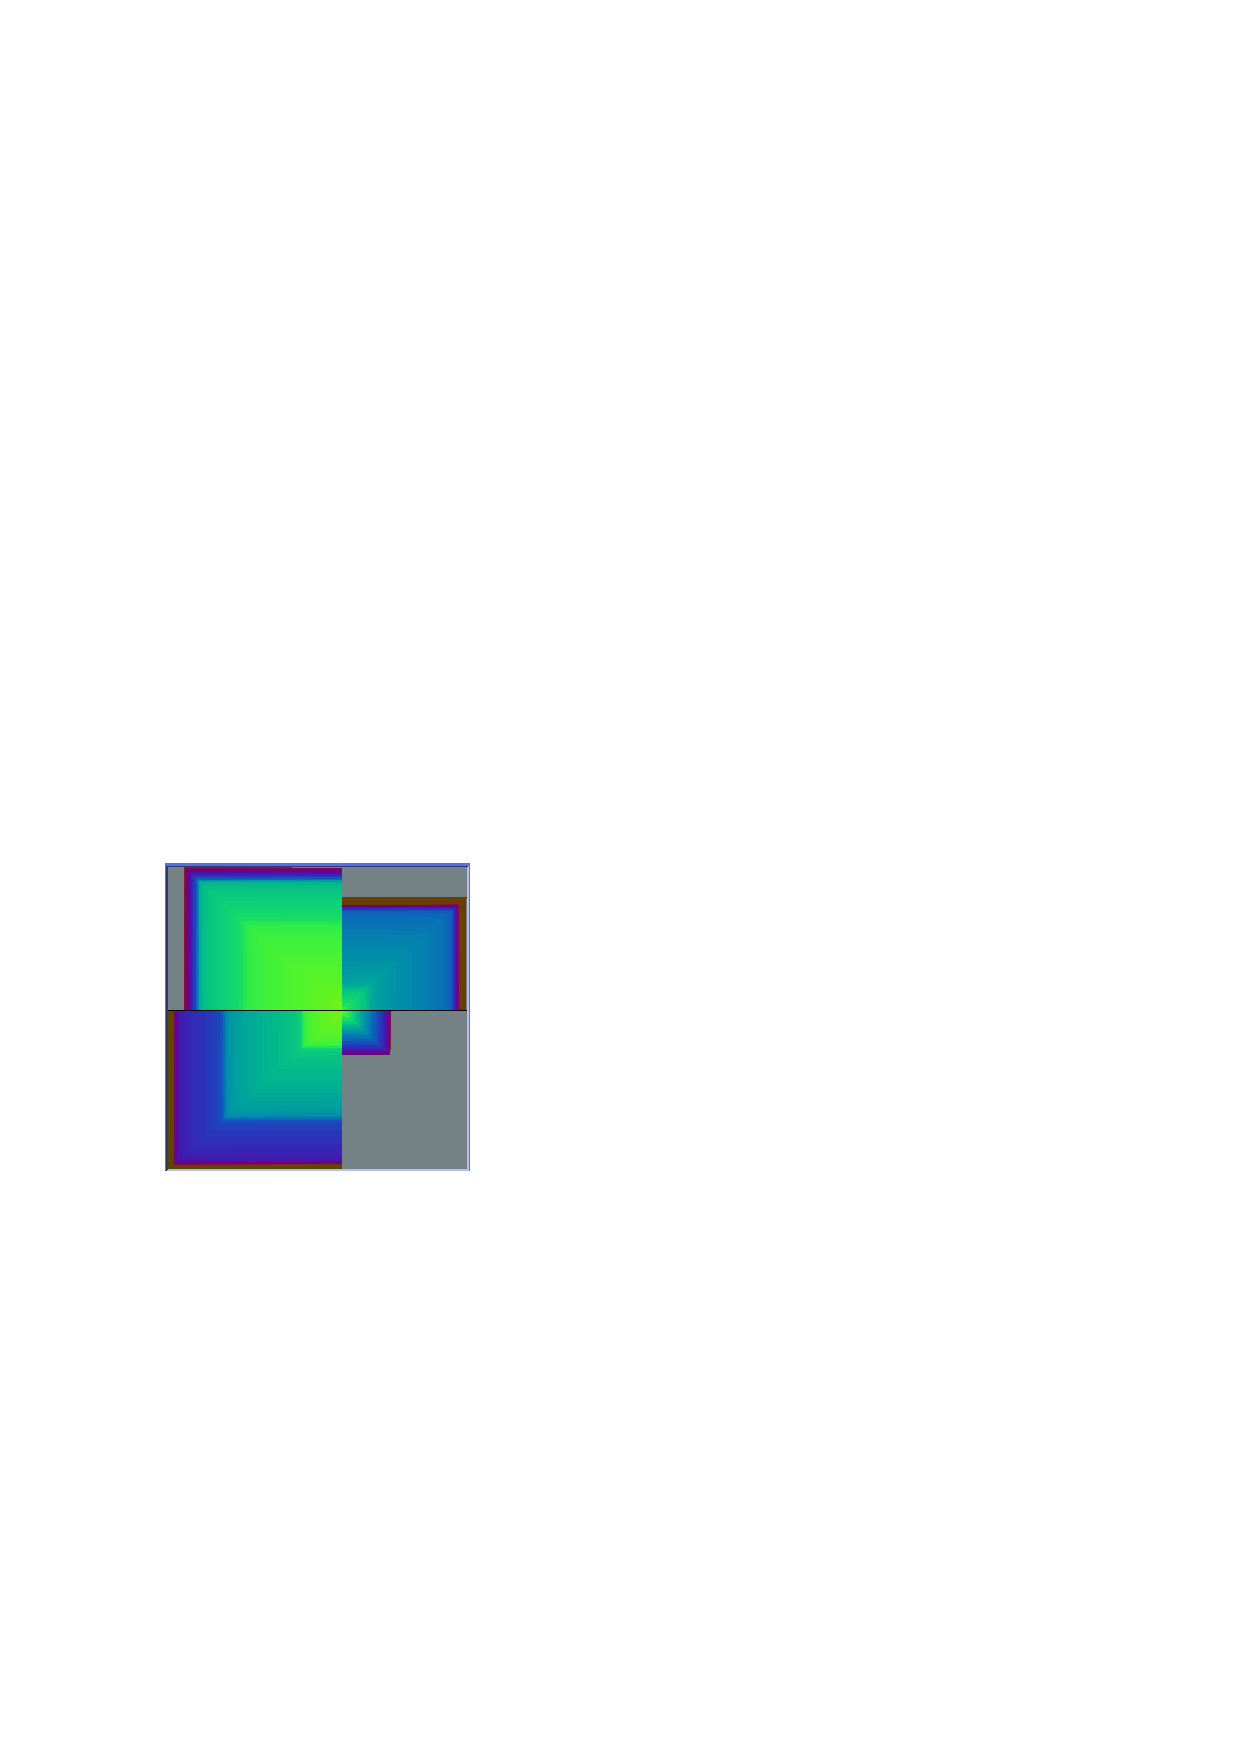
\includegraphics [width=\linewidth]{figures/pixel_keim_axes.pdf}
    \captionof {figure}{Axes \cite{keim94pixel}}
    \label{fig:pixel-axes}
}
\hfill
\parbox [h]{0.35\textwidth }{
    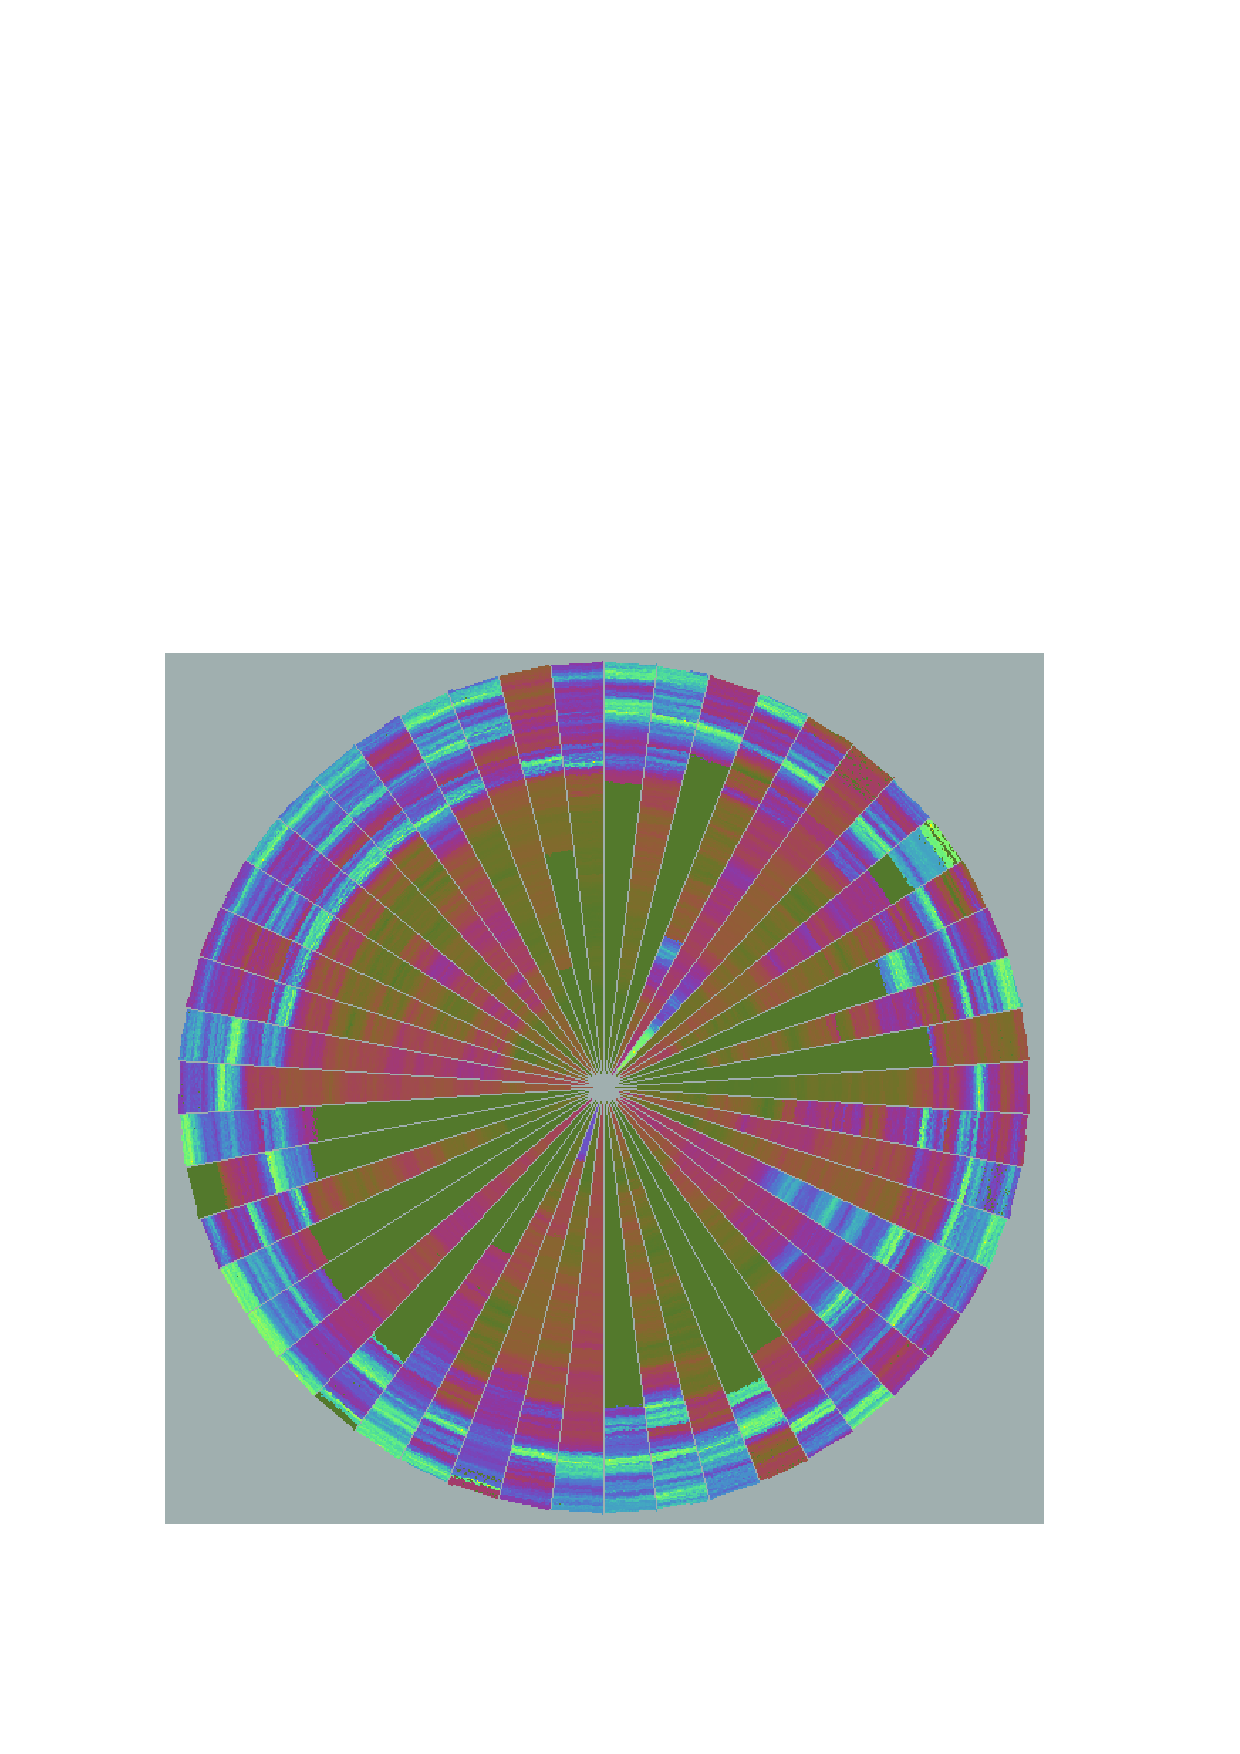
\includegraphics [width=\linewidth]{figures/pixel_keim_circle.pdf}
    \captionof {figure}{Circle \cite{Ankerst96circlesegments}}
    \label{fig:pixel-circle}
}


\item \textbf{Geometric techniques \& Diagrams}

\textit{Geometric techniques} produce useful and insightful visualization by using geometric transformations and projections of the data. \textit{Diagrams} are algorithmically drawn graphics that visualize data. This section lists a selection of geometric techniques for multivariate data presented by Ke-Bing Zhang~\cite{zhang07thesis}, diagram types described by Dieter Ladenhauf~\cite{ladenhauf12dia} and related examples found in additional literature and on the web as stated in the individual references.

\begin{itemize}

\item \textit{Line charts} visualize data as lines by connecting data points of the corresponding values. They are used to display trends over time. Figure \ref{fig:dia-map-sparklines} illustrates surface temperature anomalies from NASA's GISS\footnote{NASA Goddard Institude for Space Studies \url{http://www.giss.nasa.gov/}} as a \textit{Sparkline} map~\cite{web:sparkmaps}. The Sparkline is a reduced line chart without axes and coordinates. It presents the general shape of variation in a simple and highly condensed way~\cite{wiki:sparkline}.

\item \textit{Bar charts} express data values by vertical or horizontal bars, in which the length of a bar indicates the data value. Figure \ref{fig:dia-map-barchart} shows an example from UgandaWatch\footnote{UgandaWatch: \url{http://www.ugandawatch.org/}}, which displays economic indicators per region for the country Uganda.

\parbox [h]{0.4\textwidth }{
    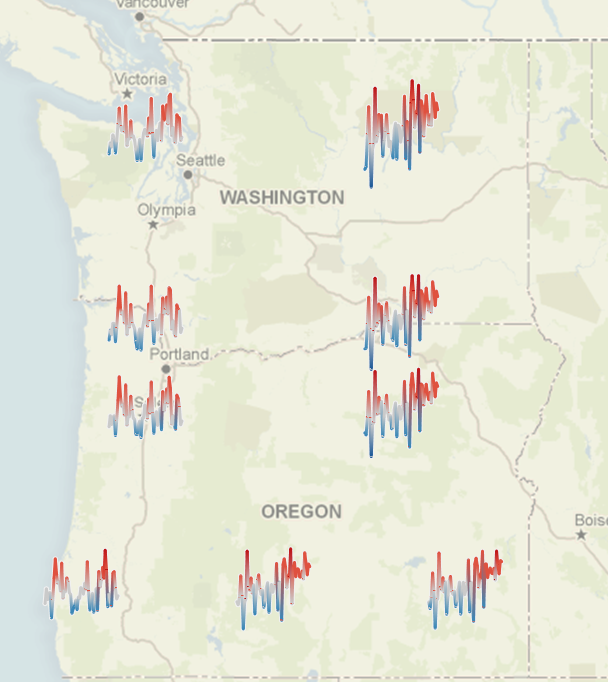
\includegraphics [width=\linewidth]{figures/dia_map_sparklines.png}
    \captionof {figure}{Sparkline map\protect\footnotemark}
    \label{fig:dia-map-sparklines}
}\footnotetext{Sparkline map example: \url{http://www.tableausoftware.com/about/blog/2008/08/sparklines-maps}}
\hfill
\hspace{0.5cm}
\parbox [h]{0.4\textwidth }{
    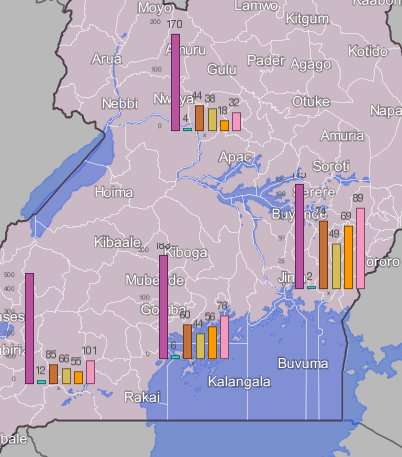
\includegraphics [width=\linewidth]{figures/dia_map_barchart.png}
    \captionof {figure}{Bar chart map\protect\footnotemark}
    \label{fig:dia-map-barchart}
}\footnotetext{UgandaWatch bar chart example: \url{http://www.ugandawatch.org/}}


\item \textit{Pie charts} use a circle divided into sectors for expressing the proportional significance of data values. Variants of pie charts include \textit{doughnut charts}, \textit{three-dimensional pie charts} and \textit{multi-level pie charts}. Also, the \textit{polar area diagram} introduced in figure \ref{fig:map-type-standard-wind} is a special kind of pie chart and a further development of the \textit{Bat's wing diagram} by Florence Nightingale~\cite{night98bart}.

Figure \ref{fig:dia-map-piechart} depicts a pie chart map example from the Kartograph\footnote{Kartograph \url{http://kartograph.org/}} framework. It shows unemployment rates in Spain, providing an effective way to display ratios as opposed to a chloropeth map, where the user usually needs to consult a legend to understand the actual data values.

\item \textit{Container shapes} such as \textit{bounding boxes} and \textit{hulls} are an alternative to iconic displays as they can show the area covered by clusters~\cite{Delort10vis}. The Leaflet.markercluster library visualizes the convex hull of a cluster to indicate the covered area on mouse-hover. Marco Cristani et al~\cite{Cristani08geoimagemaps} use a hull-based technique for visualizing clusters from a geo-located image database on a map. As illustrated in figure \ref{fig:dia-map-hull}, each cluster is represented by a hull that marks the boundaries of the area and contains a representative image of the clustered set of images.


\parbox [h]{0.4\textwidth }{
    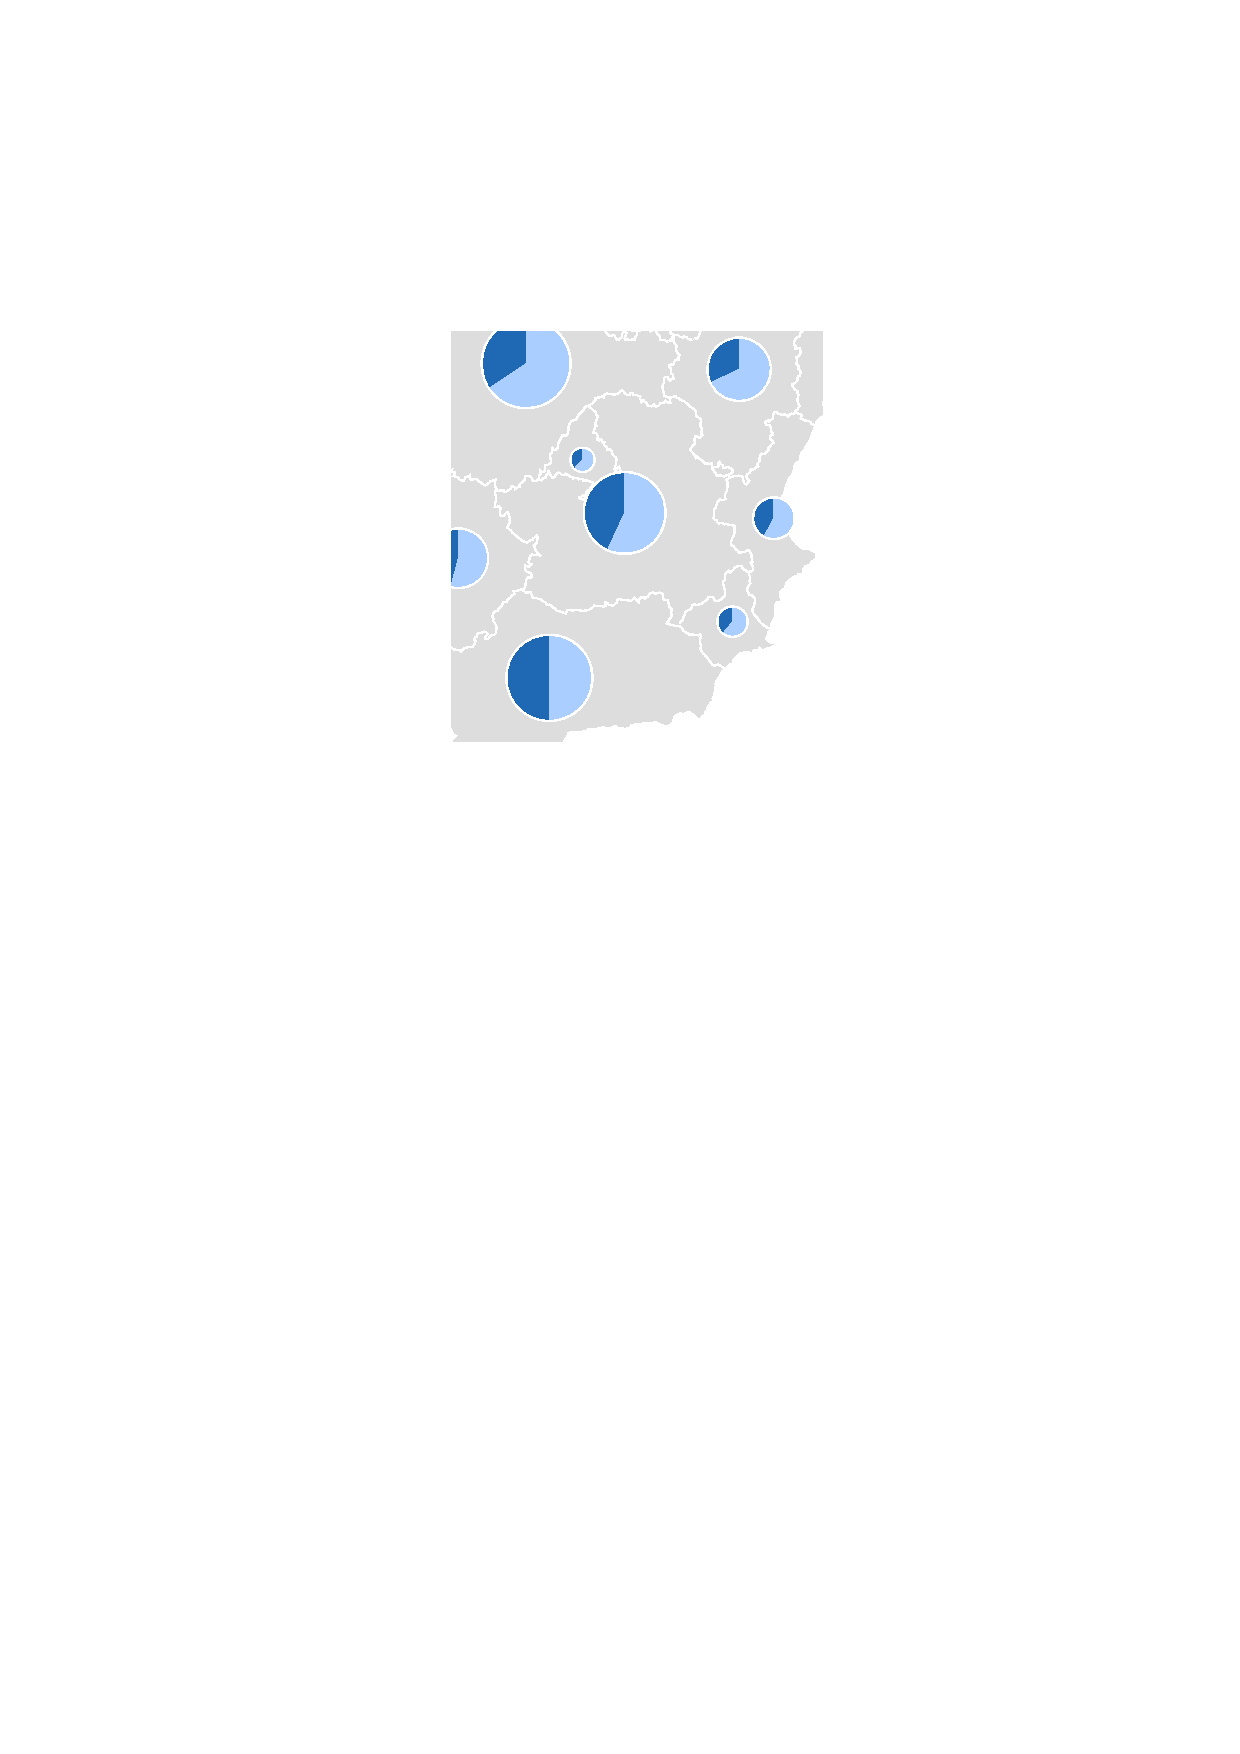
\includegraphics [width=\linewidth]{figures/dia_map_piechart.pdf}
    \captionof {figure}{Pie chart map\protect\footnotemark}
    \label{fig:dia-map-piechart}
}\footnotetext{Pie chart map example from Kartograph: \url{http://kartograph.org/showcase/charts/}}
\hfill
\hspace{0.5cm}
\parbox [h]{0.4\textwidth }{
    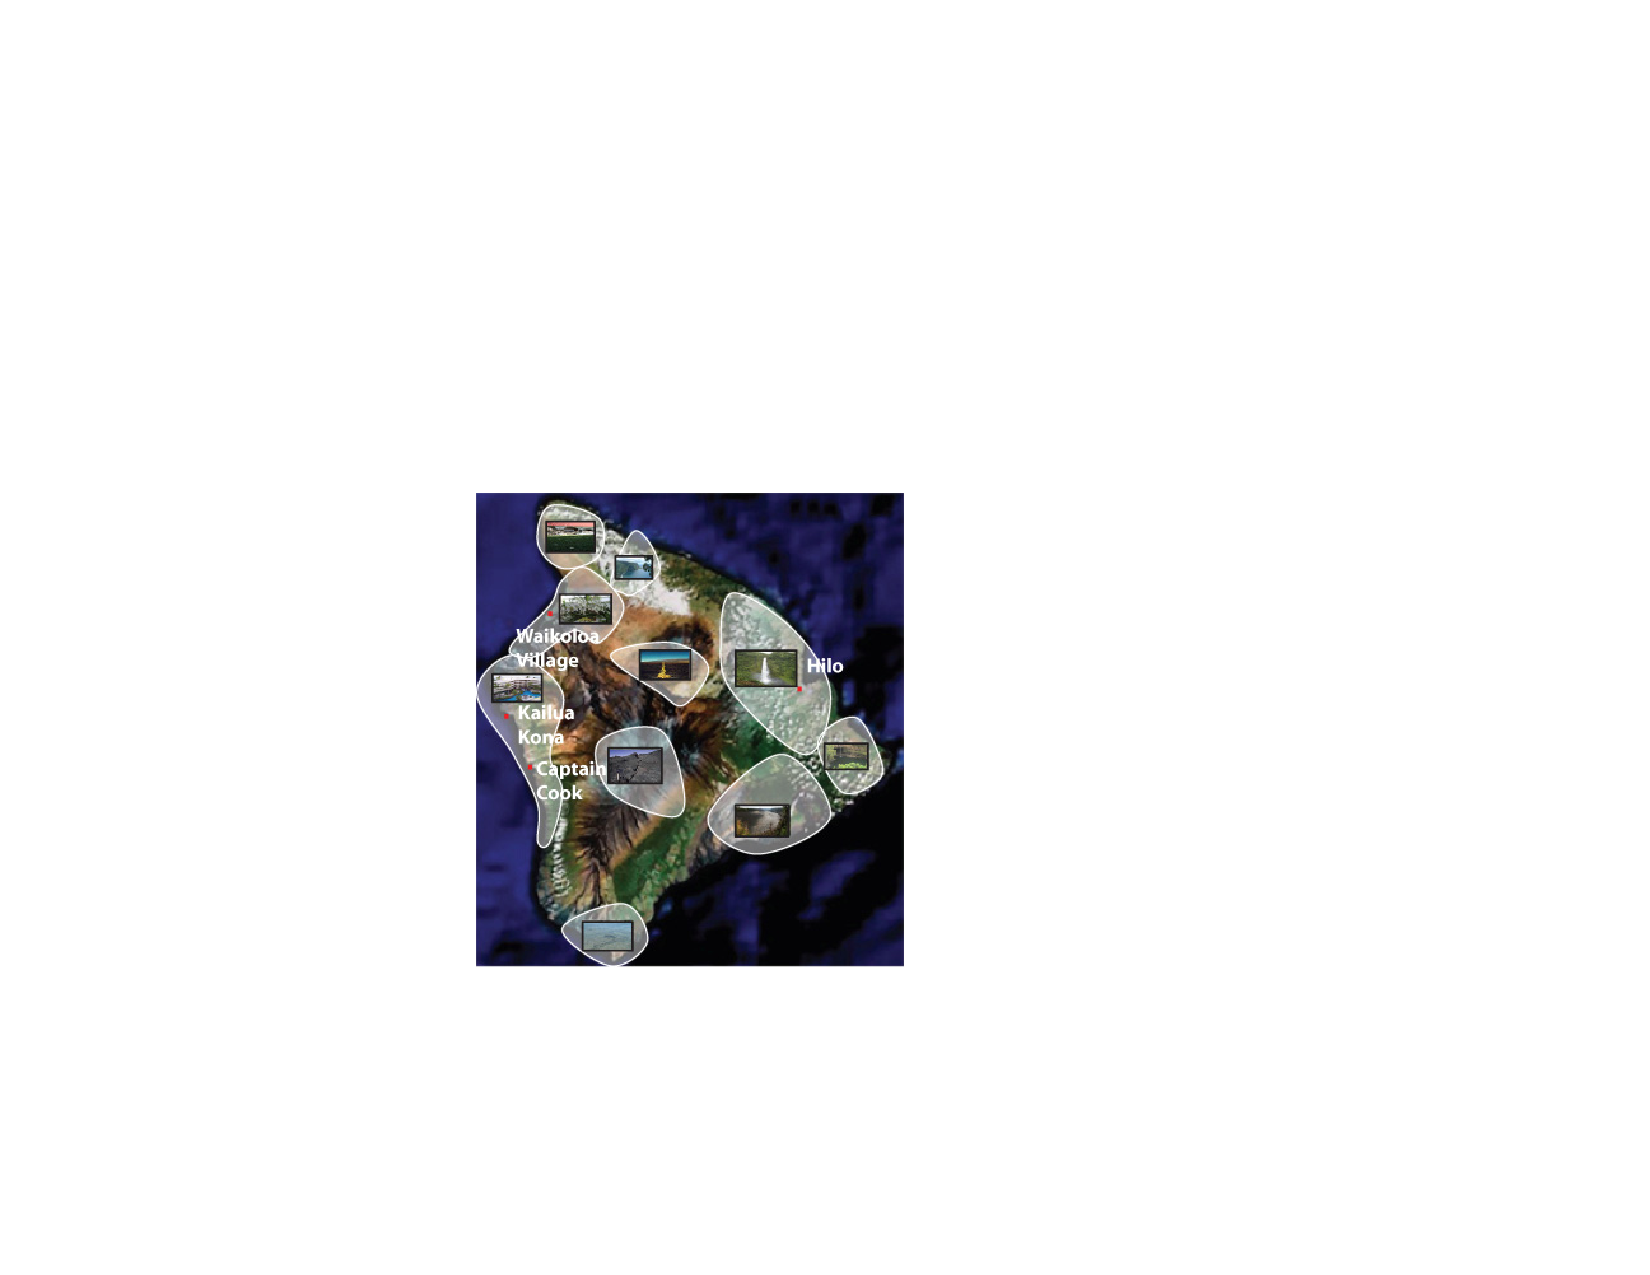
\includegraphics [width=\linewidth]{figures/dia_map_hull.pdf}
    \captionof {figure}{Convex hull map\protect\footnotemark}
    \label{fig:dia-map-hull}
}\footnotetext{Convex hull map example from \cite{Cristani08geoimagemaps}}



\item Further chart types that can possibly used for visualizing clusters on a map include \textit{Area charts} and \textit{Star plots}~\cite{ladenhauf12dia} or more complex ones like \textit{Parallel coordinates}, \textit{Scatterplots}, \textit{Treemaps}~\cite{zhang07thesis} or the \textit{Contingency Wheel++} \cite{VAST2012}. \textit{Bristle maps} are an interesting approach for visualizing spatio-temporal data on a map. Basically, histograms of the data are rendered onto linear map elements. If the data permits a mapping from aggregates to spatial line data, such a visualization technique could be of interest~\cite{bristle}.

\end{itemize}

\end{itemize}

This concludes the investigative enumeration of cluster visualization techniques for maps. It is by no means a complete, but rather an exemplary listing that may provide a starting point when researching visual means of presenting clustered data on a map.

An interesting publication by Andrienko et al~\cite{andrienko2012sca} presents a complex system for place-oriented analysis of movement data. This goes beyond the use case of simply visualizing clustered data on a slippy map, but it is a good show case for how effective the presentation of spatio-temporal data using a combination of techniques can be. \textit{Time graphs}, \textit{mosaic diagrams}, \textit{space-time cubes} and \textit{table lens displays} are used to create a powerful tool for inspecting movement data on maps.



\section{Evaluation of visualization techniques for clusters on a map}
\label{chapter:eval-vis}

This chapter summarizes the main visualization examples presented in the previous chapters. An evaluation of techniques for visualizing clusters on maps is created by proposing a set of key characteristics that are considered to be significant for this kind of visualization.

Evaluating information visualization techniques is a well-known problem. Undertaking an evaluation that is capable of ``proving'' the effectiveness is impossible in many situations as it would require too many tasks, data sets, implementations and users. Ellis and Dix state exploratory analysis as the most effective approach for evaluating visualization techniques~\cite{ellis06eval, Delort10vis}. In this sense, the following evaluation should primarily be treated as exploratory and as a help for understanding how cluster visualization on maps works, rather than a final, summative conclusion of which technique is superior than another. 

\textbf{Criteria}. the following, custom criteria have been defined: \textit{category}, \textit{shows number of items within cluster} (\textit{by shape size}, \textit{by color or other}), \textit{shows cluster area}, \textit{shows extra cluster info} \textit{(extra cluster info complexity}). Some criteria contain sub-criteria which are stated within parentheses.

In chapter \ref{chapter:foundations-vis}, three taxonomies have been introduced: \textit{visual variables}, a \textit{classification of visual data exploration techniques} and a \textit{clutter reduction taxonomy}. An attempt to classify the different visualization techniques for representing clusters on maps according to classes introduced by these taxonomies didn't feel valid. Some criteria are too general while others are too specific to actually matter for visualizing clusters on maps, so the resulting data would not have much value. Similarly, a classification based on all \textit{visual variables} would have become very complex. As the presented visualization examples describe general concepts, there are many possible variations that would increase the data set even more. It is still helpful to rely on the aesthetic attributes for a better understanding of how each visualization is constructed. Especially the \textit{shape}, \textit{size} and \textit{color} attributes are considered to have a strong effect on visualizing clusters on maps and are therefore included within the evaluation.

An explanation of each criterion follows:

\begin{itemize}

\item \textbf{category}: Determines the type of visualization technique being evaluated. Possible values are \textit{type of map} (see chapter \ref{chapter:map-vis}), a visualization \textit{example}, as well as abbreviations for cluster visualization techniques (see chapter \ref{chapter:cluster-vis}): \textit{glyph}: Icon-based, Glyphs, \textit{pixel}: Pixel-oriented techniques and \textit{geom}: Geometric techniques \& Diagrams.

\item \textbf{shape}: Defines the type of shape being used for the visualization of clusters on the map. For example \textit{circle} or \textit{area}. Refer to the visual variable shape in chapter \ref{chapter:vis-variables}. 

\item \textbf{shows \# of items within cluster}: If the visualization provides an indicator of the amount of items per clusters. This relates to the `can see overlap density' criterion of the clutter reduction taxonomy, see \ref{clutter-reduction}. Two sub-criteria are used to differentiate between visual means of encoding the number of items within clusters: 

\begin{itemize}

\item \textbf{by shape size}: classifies visualization techniques that use the shape size for indicating the number of items within clusters.

\item \textbf{by color or other}: classifies visualization techniques that use color or other visual indicators to describe the number of items within a cluster.

\end{itemize}

\item \textbf{shows cluster area}: Determines, if the visualization indicates the spatial area that is covered by the cluster or the items within a cluster.

\item \textbf{shows extra cluster info}: Besides the two characteristics of number of items within a cluster and the cluster area, the technique might provide means of visualization additional information of clusters such as aggregates. 

\begin{itemize}

\item \textbf{extra cluster info complexity}: This sub-criterion expands of an intuitive notion of complexity that can be visualized as extra cluster info by the technique. \textit{low} indicates a maximum of three dimensions. \textit{medium} is used to describe up to 12 dimensions of additional data and \textit{high} classifies cluster visualization techniques that go beyond this number of dimensions.

\end{itemize}

\end{itemize}

\begin{figure}[h]
  \begin{center}
    \hspace*{-1.5cm}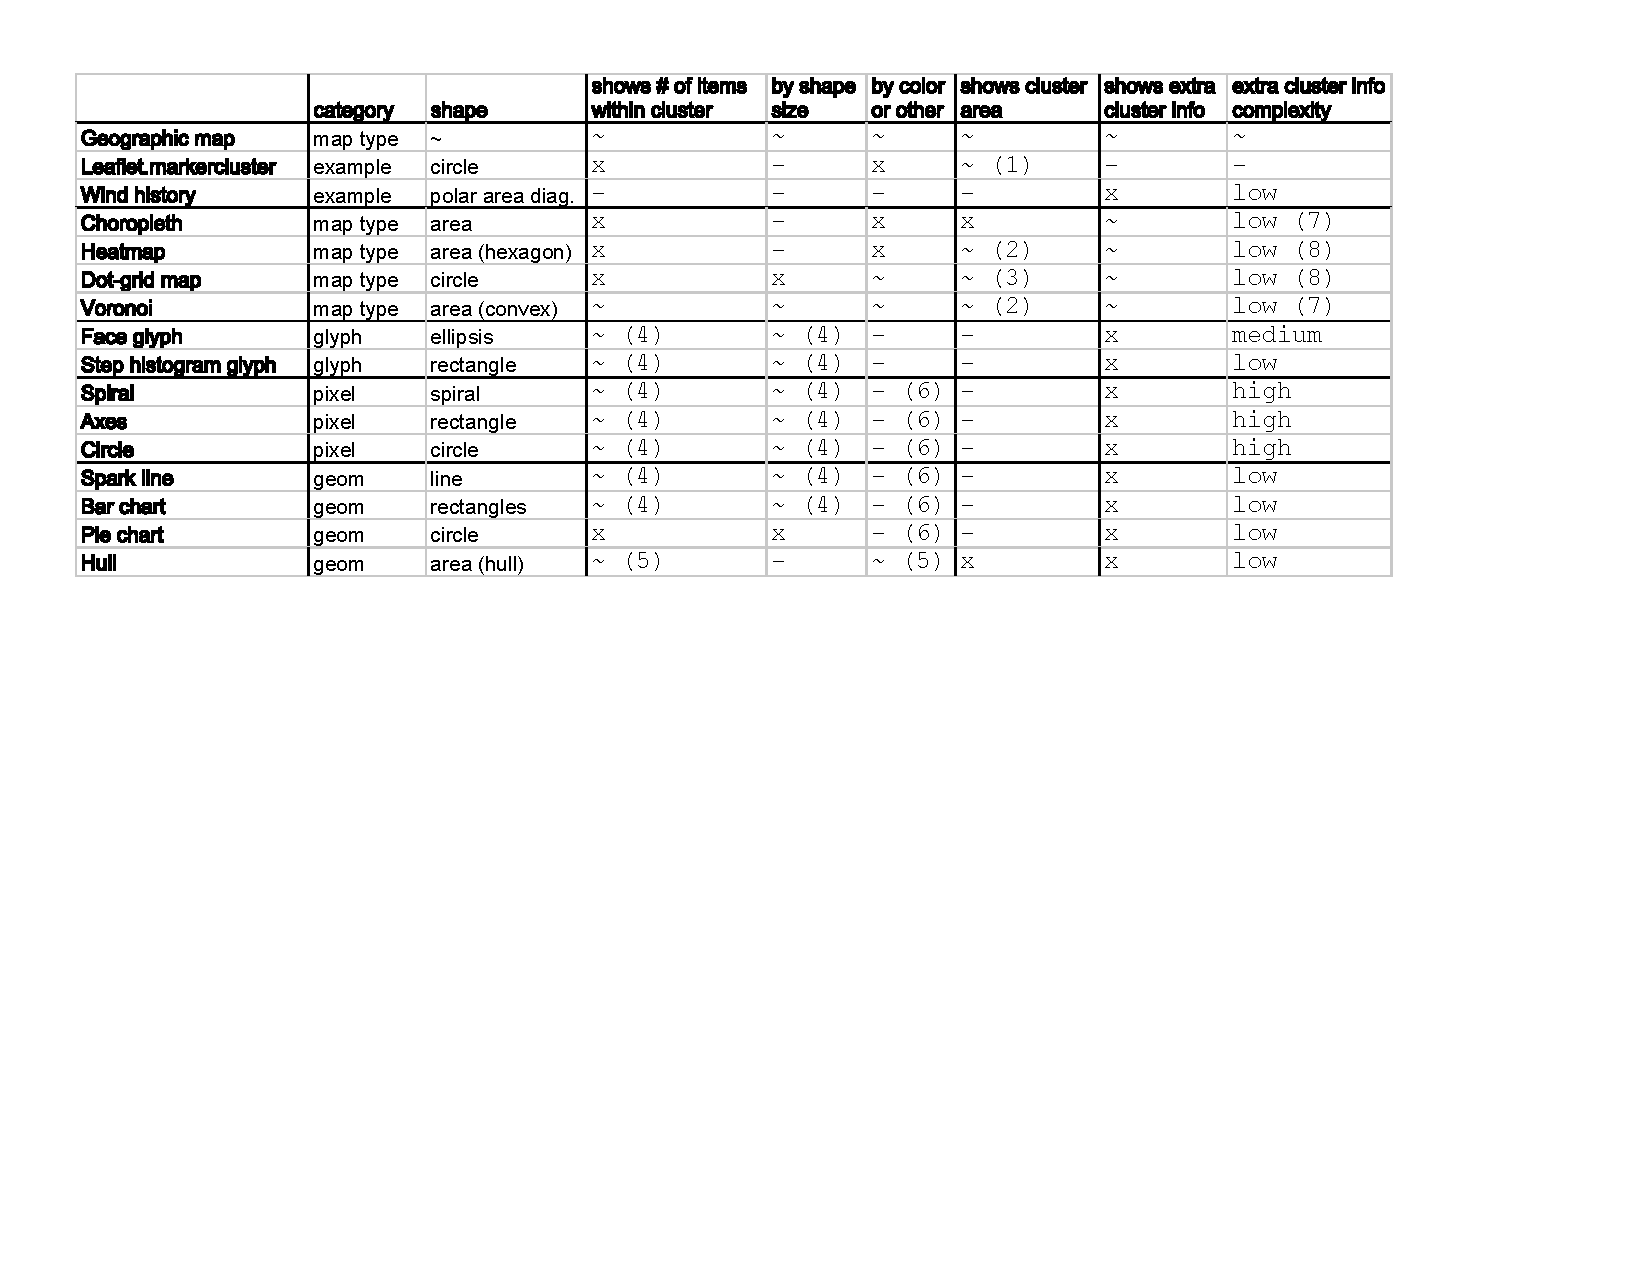
\includegraphics[width=1.2\textwidth]{figures/vis_evaluation.pdf}
    \caption{Evaluation of visualization techniques for clusters on a map. Legend:~`x':~yes,~`\textasciitilde': possibly, `-': no. Numbers in parentheses reference additional notes within the accompanying text.}
    \label{fig:vis-eval}
  \end{center}
\end{figure}

The results of the evaluation of visualization techniques for clusters on a map based on the stated criteria are illustrated in figure \ref{fig:vis-eval}. Note that the classifications for each technique being evaluated primarily represent the according examples shown in the previous chapters. Where it seemed obvious, the optional possibility of fulfilling a criterion has been marked as such. As an extreme example, the geographic map as its general concept has been marked with the optional possibility of fulfilling each criterion. It is up the the actual implementation to satisfy them individually. While the Leaflet.markercluster example provides a visual indicator for the number of items within clusters, the wind history example doesn't.

Some classifications contain a number referring to additional notes as presented in the following: (1) The Leaflet.markercluster example shows cluster on demand, based on user interaction. By mouse-hovering over an item, it will display the convex hull of the items being clustered. (2) In the case of the binned heat map example and the Voronoi map, cluster areas are approximated by the tessellation which is part of the clustering algorithm, see figure \ref{fig:map-type-binning} and \ref{fig:map-type-voronoi}. (3) The dot-grid map doesn't provide a mean of showing cluster areas by themselves, but the density of items still supports the notion of recognizing cluster areas, see figure{fig:map-type-dotgrid}. (4) For various visualization techniques, the amount of items within a cluster could be visualized by simply scaling the visual entity. (5) The hull example uses an area shape defined by the data, similarly to the choropleth map. Without a distortion technique, the shape therefore can't be used to indicate the number of items within a cluster. Still, a non-shape visual aspect like color could be used as an indicator. (6) In the case of pixel-oriented techniques and the provided chart examples, the color attribute will likely be used for showing extra cluster info instead of indicating the number of items within a cluster. Modifying the shape size can be used as an alternative in this cases. (7) The choroleth and voronoi map examples would rely on representing extra information within the defined area and therefore rely on the.variation of visual variables related to color and texture. (8) The same restrictions as in the previous note apply, but for even smaller areas.

Map visualization types and cluster visualization techniques for maps have been introduced and were summarized within the given evaluation.





\chapter{Discussion}
\label{chapter:discussion}

The previously presented evaluation classifies 7 different map visualizations that contain clusters (5 map types and 2 examples), as well as 9 cluster visualization techniques (2 glyphs, 3 pixel-based and 4 geometric / diagrams). Each visualization has been evaluated against a limited set criteria which are considered as important for showing clustered, multi-variate data on maps.

All visualizations, with the exception of the Wind history example, fulfill the primary criterion of \textbf{being able to indicate the number of items within clusters}. This makes sense, as in many cases \textit{seeing overlap density} is an important feature of the visualization to indicate the amount of overplotting and tell the user an estimate of what to expect within the cluster. In the case of the Wind history example this is not necessary because all clusters are of the same size and visualize their inner data ratio as part of the polar area chart. Given the many classifications of ``possibly'' and considering the presented examples, it seems like fulfilling this criterion heavily depends on the needs of the use case. The fact, that all evaluated visualization techniques support showing cluster sizes, apparently correlates with their selection process. Naturally, those visualization approaches have been evaluated that seemed logical for visualizing clustered data. 

On the contrary, few visualization techniques fulfill the criterion of \textbf{showing the cluster area}. The presented glyphs, pixel-based and diagram techniques do not have this feature as their shape is predefined. On the other hand, the Hull example indicates that a shape that indicates area can also be combined with an arbitrary shape inside.

While most cluster visualization techniques fail at indicating areas, they are perfectly suited for \textbf{showing extra cluster info}. Glyphs, geometric-techniques and diagrams appear suitable for visualizing cluster info of lower complexity while pixel-based techniques are geared towards multi-variate data of higher complexity.


Given the general discussion of the study results, a practical evaluation of the Geocluster concludes the discussion.

\section{Geocluster visualization}
\label{chapter:geocluster-vis}

Geocluster\footnote{\url{http://drupal.org/project/geocluster}} is a server-side clustering implementation for mapping with Drupal based on Geohash. Refer to the complete thesis on Geocluster for an explanation of related concepts as Drupal, the Drupal mapping stack, Bounding Box strategies etc. \cite{geocluster-thesis}. Two visualizations for Geocluster have been implemented:

\begin{itemize}

\item \textbf{Geocluster default visualization}

A simple Geocluster visualization component has been built to support the display of clustered markers on interactive maps based on the output of the server-side clustering implementation. It extends the Bounding Box strategy of the Leaflet GeoJSON module in oder to create numbered markers that visualize the cluster sizes. Clicking on a clustered marker will zoom into the map in order to explore the data on a more granular level. Figure \ref{fig:map-clustered} demonstrates an example screenshot of the Geocluster visualization. Compare this with an unclustered map, containing the same amount of items in figure \ref{fig:map-unclustered}.


\hspace*{-1.5cm}\parbox [h]{0.5\textwidth}{
    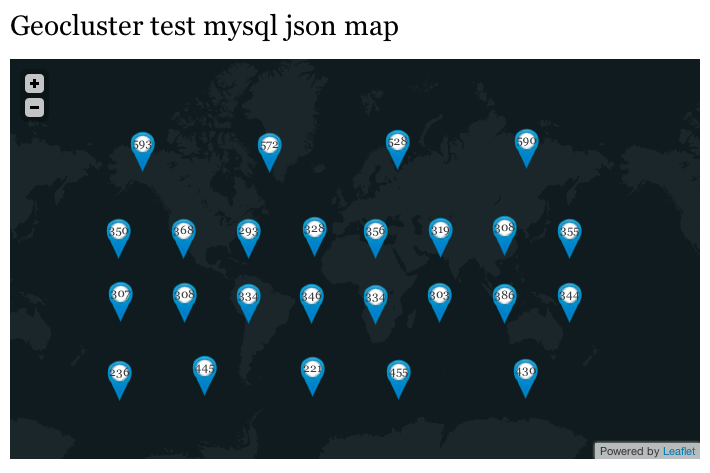
\includegraphics [width=\linewidth]{figures/map_clustered.png}
    \captionof {figure}{Geocluster visualization}
    \label{fig:map-clustered}
}
\hfill
\hspace{0.5cm}
\parbox [h]{0.5\textwidth }{
    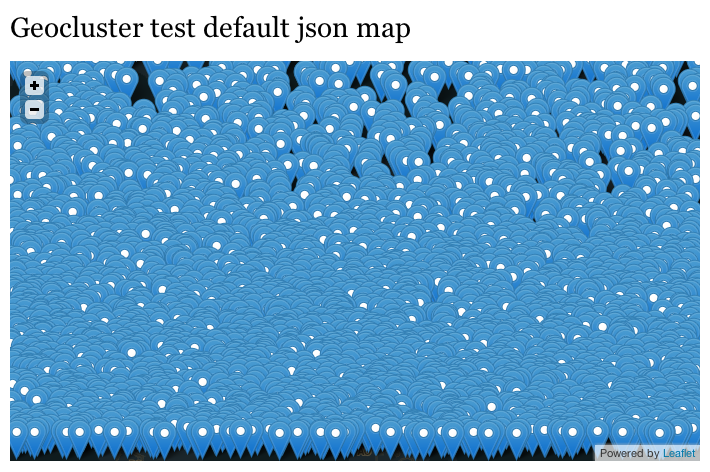
\includegraphics [width=\linewidth]{figures/map_unclustered.png}
    \captionof {figure}{Unclustered Leaflet map}
    \label{fig:map-unclustered}
}


The visualization component of Geocluster is based on a GeoJSON-feed provided by the server-side clustering implementation. It uses the JavaScript Bounding Box strategy to dynamically update results for the current viewport after zooming or panning the map. The cluster visualization is very simple and based on a code snippet for numbered markers on github\footnote{\url{https://gist.github.com/comp615/2288108}}.


\item \textbf{GeoRecruiter}

\begin{figure}[h]
  \begin{center}
    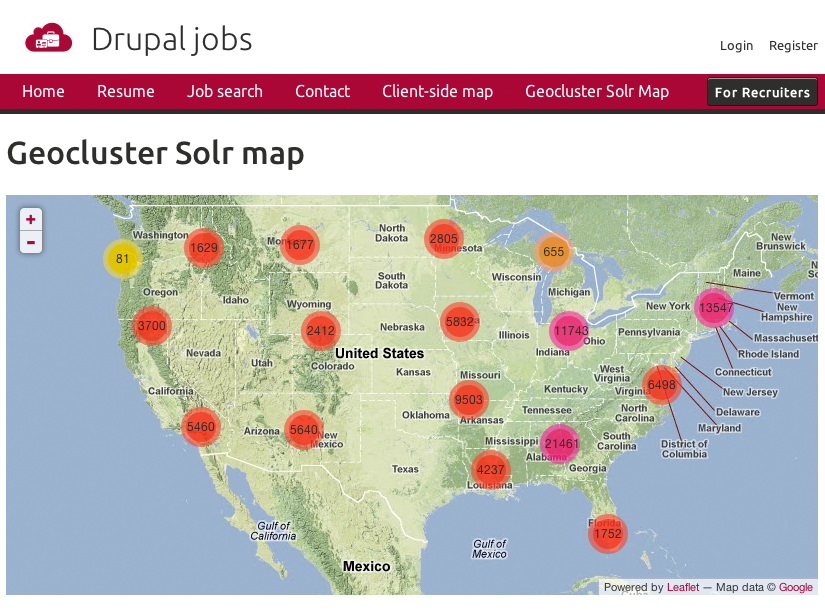
\includegraphics[width=1\textwidth]{figures/drupaljobs_geocluster_solr.png}
    \caption{Screenshot of map that visualized job search results on a map using Solr-based clustering on a Drupaljobs test installation.}
    \label{fig:drupaljobs-geocluster-solr}
  \end{center}
\end{figure}

A practical use case for server-side geo clustering has been implemented for the Recruiter job board solution. It supports spatial search capabilities of the Recruiter distribution by visualizing a large amount of job offers on e-recruitment websites. The prototype being discussed has been developed based on a copy of the Drupaljobs website\footnote{\url{http://drupaljobs.epiqo.com}}.

\begin{quote}
\textit{Recruiter} is a Drupal distribution for building Drupal based e-recruitment platforms. Users can register either as recruiter and post job classifieds or they can register as applicants and fill out their resume. A faceted search helps users to find jobs and possible job candidates.\footnote{\url{http://drupal.org/project/recruiter}}. \textit{Drupaljobs} is provided as a show case for the Recruiter distribution. Its base features allow to create and search for job offers by companies as well as resumes of registered applicants on the e-recruitment platform.
\end{quote}


A map visualizes the clustered job search results. In order to enhance the representation of clusters and to experiment with interaction, the CSS styles of client-side clustering library Leaflet.markercluster have been adapted and extended with additional colors for large clusters. A visualization of a map within the Drupaljobs test installation is provided in figure \ref{fig:drupaljobs-geocluster-solr}.




\end{itemize}

\section{Visual evaluation of Geocluster}

Two visualizations have been provided: first, the Client-side Geocluster Visualization component as visualized in figure \ref{fig:map-clustered} and second, an alternative visualization similar to the Leaflet.markercluster library for the GeoRecruiter use case, see figure \ref{fig:drupaljobs-geocluster-solr}.

Both implementations fulfill most of the clutter reduction criteria from chapter \ref{clutter-reduction}:

\begin{enumerate}

\item \textit{Overlap} is avoided by visualizing a non-overlapping clustering of points, as created by geohash-based clustering algorithm of Geocluster.

\item \textit{Spatial information} is expressed as an aggregate of latitude and longitude values for each cluster, approximating its centroid. One problem with the current implementations is, that clusters aren't ``stable''. In some experiments, changes to the bounding box will cause a change of cluster assignment. Intuitively, this leads to confusion of the user and should be investigated upon further. 

\item The Leaflet Bounding Box strategy implementation allows to \textit{localize} the view by panning and zooming and therefore reduce the display to a specific region.

\item \textit{Scalability} is provided by the underlying clustering algorithm, as evaluated in the previous section.

\item The configuration options of Geocluster allow to \textit{adjust} the minimum distance between clusters. Additional configuration options are provided by the Views integration of the Geocluster module. Still, the configuration options could be expanded for example to control visual parameters of clusters. 

\item The criterion of \textit{showing point/line attributes} is fulfilled only in a very limited way. Both implementations are currently restricted to displaying the number of items within a cluster as the only aggregate value. In order to support complex visualization techniques for multivariate data as discussed in chapter \ref{chapter:cluster-vis}, the clustering implementation needs to provide the required, aggregate values of the underlying data.

\item As explained in the discussion of the \textit{discriminating points/lines} criterion, its definition seems unclear. Clustered items and individual points are visualized in a different way, which can be seen as a fulfillment. On the other hand, the visualization currently doesn't provide any means of inspecting clusters. Only a list of identifiers of the items within a cluster is provided. Based upon the identifiers, a popup could be used to visualize the items a in more detailed way.

\item With regards to \textit{overlap density}, the number of items within clusters is indicated by both visualizations, but using different means. The Geocluster visualization doesn't make use of visual attributes like size or color, instead it creates a marker glyph that contains the number of items using textual representation. The GeoRecruiter prototype uses a color ramp that indicates low cluster densities from green and yellow to high densities indicated by tones of red and violet.

\end{enumerate}

\begin{figure}[h]
  \begin{center}
    \hspace*{-1.5cm}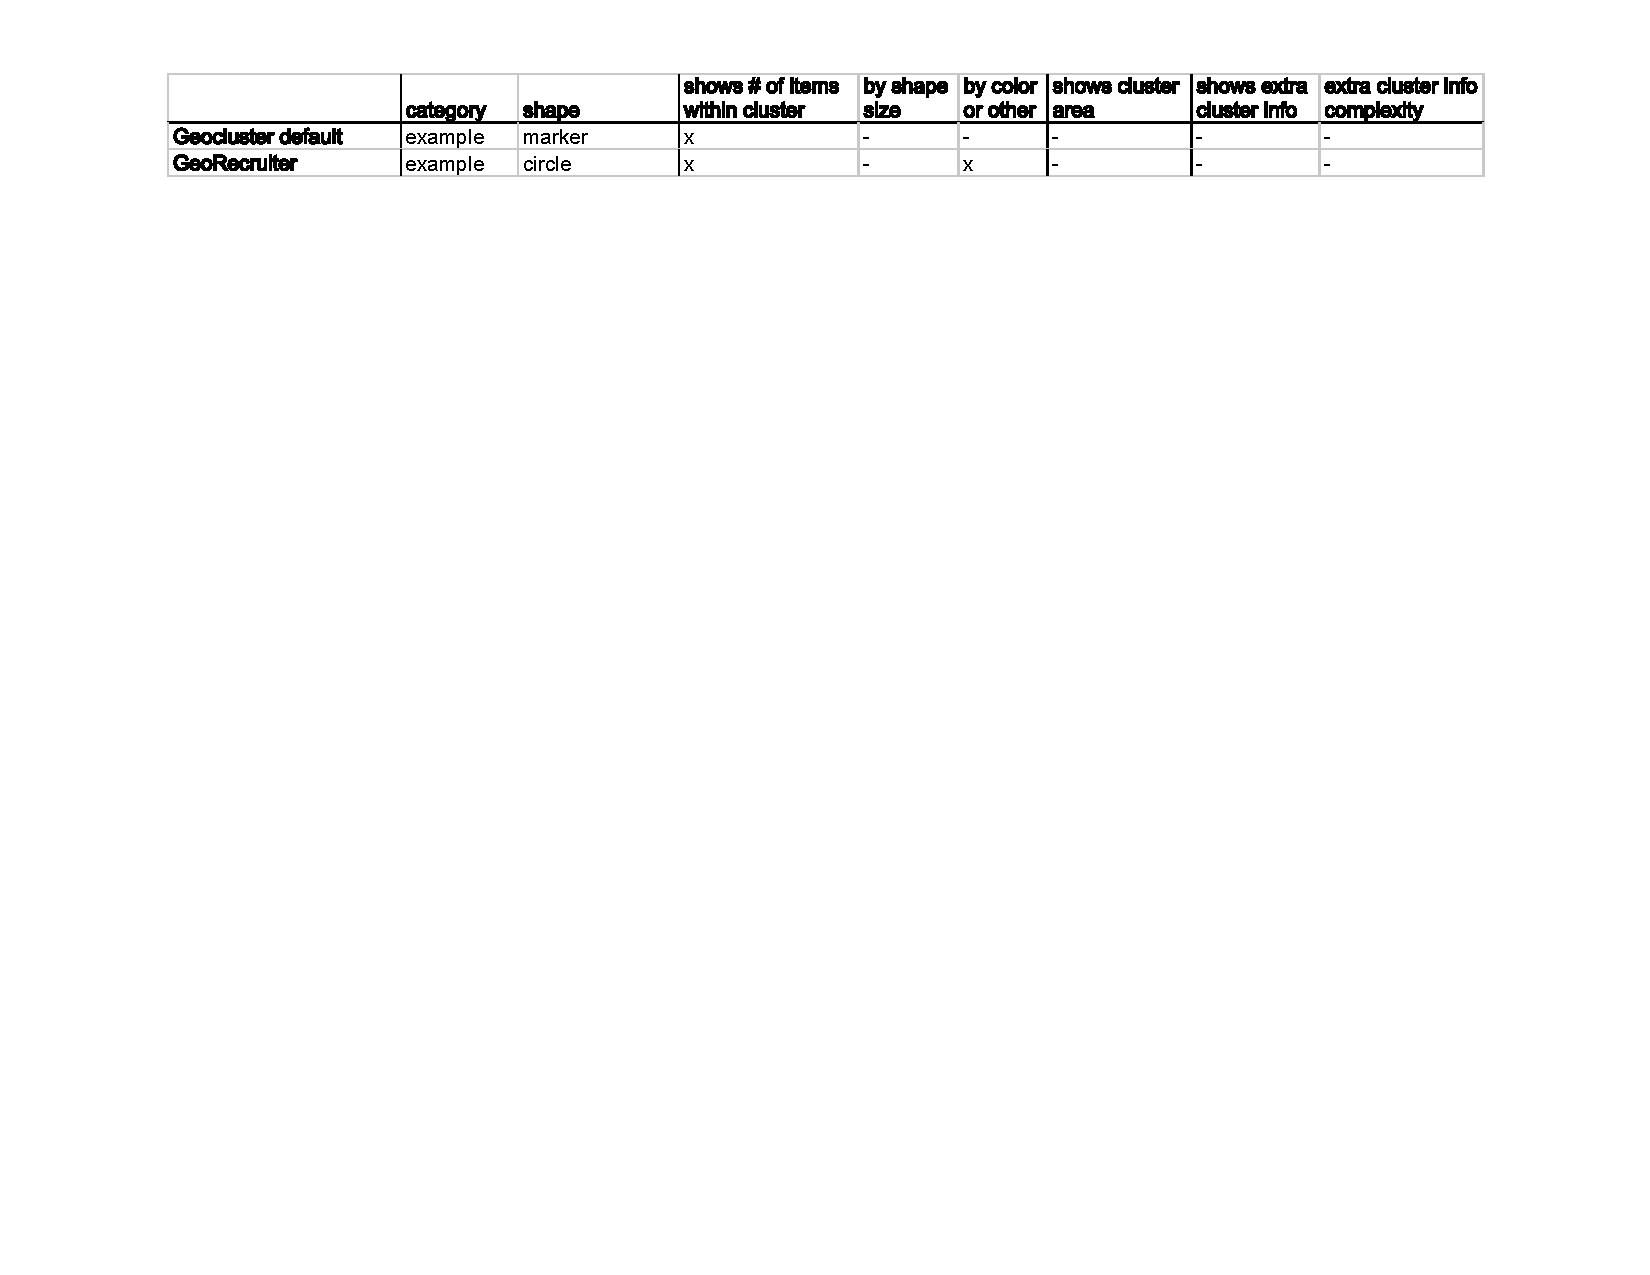
\includegraphics[width=1.2\textwidth]{figures/vis_eval_geocluster.pdf}
    \caption{Evaluation of Geocluster visualization techniques for clusters on a map. Legend:~`x':~yes,~`\textasciitilde': possibly, `-': no.}
    \label{fig:vis-eval-geocluster}
  \end{center}
\end{figure}

Next, the evaluation of visualization techniques for clusters on map presented in \ref{chapter:eval-vis} is applied to the two Geocluster implementations as illustrated in figure \ref{fig:vis-eval-geocluster}. It reiterates some key aspects identified by the previous discussion of clutter reduction criteria.

\textbf{Cluster sizes}: Both visualizations show the number of items within a cluster, but only the GeoRecruiter example uses color and none of them encodes the size of a cluster into the shape size. As naturally, a cluster with more items can be visualized larger than smaller clusters, the algorithm could be improved for growing clusters by their size. The bigger size of a cluster would therefore reduce the distance to its neighbor clusters, potentially merging additional neighbors into it. Andrew Betts describes a similar approach under the term \textit{``Grid based viral growth argorithm''}~\cite{web:clustering-google}.

\textbf{Cluster areas}: Neither implementation provides a visual indicator for showing cluster areas. Again, the server-side clustering implementation would need to provide this information. Instead, for performance reason only the number of items within clusters is provided as aggregate values.

\textbf{Extra cluster info}: Similarly, no additional data about aggregates within clusters is exposed by the clustering implementation. This might suffice the use case of clustering points on maps for reducing clutter, but potentially hides a lot of information that could be displayed as part of the cluster visualization. 

On a note on performance of the interaction, for low zoom levels, the roundtrip to the server for fetching a separate clustered result on every bounding box change can be an overhead. Christopher Calid proposes a way of ``Progressively enhance server-side with client-side clustering''\footnote{\url{http://drupal.org/node/1914704}}. The intention is to switch from server-side clustering at higher zoom levels to client-side clustering for lower zoom levels.



\section{Conclusions}

A simple taxonomy for classification of cluster visualization techniques for maps has been presented and applied to a selection of techniques and examples. For the particular use case of web maps, visualizing \textit{cluster sizes} was proposed as a primary goal for displaying clusters, followed by \textit{showing the cluster area} and \textit{showing extra cluster info}. The techniques have been enumerated and evaluated from two different view points: \textit{map visualization types for clusters}. In this way, a structured overview of existing approaches could be given.

The discussion of the practical implementation of Geocluster visualization for server-side clustering with maps illustrates some a major difference between the visualization of the same dataset. Indicating cluster sizes by visual means like shape size and color seems to generate a more intuitive result than simply putting numbers of cluster sizes within markers. In comparison to advanced cluster visualization techniques, the Geocluster visualization is a very simple one that doesn't show cluster areas and extra cluster infos.

A brief overview has been given by enumerating examples from different research disciplines like geovisualization, cluster visualization and chart techniques. Complex cluster visualizations seem to specific to scientific purposes of exploration and alysis of rather private audiences. Simpler cluster visualizations can be found in JavaScript mapping libraries that are used to present information to public audiences.

The study only touches on further aspects like interaction, usability and animation. Also the impact of visual variables and the exact data types being presented offers room for additional investigation. 





\newpage

 \appendix
% \chapter{Acronyms}

\begin{acronym}
\acro{AJAX}{Asynchronous JavaScript + XML}
\acro{API}{Application Programming Interface}
\acro{CMS}{Content Management System}
\acro{GNU}{GNU's Not Unix}
\acro{HTML}{HyperText Markup Language}
\acro{HTTP}{HyperText Transfer Protocol}
\acro{IDE}{Integrated Development Environment}
\acro{IT}{Information Technology}
\acro{JSON}{JavaScript Object Notation}
\acro{OASIS}{Organization for the Advancement of Structured Information
Standards}
\acro{REST}{Representational State Transfer}
\acro{RSS}{Really Simple Syndication}
\acro{UDDI}{Universal Description, Discovery and Integration}
\acro{UI}{User Interface}
\acro{URI}{Uniform Resource Identifier}
\acro{URL}{Uniform Resource Locator}
\acro{W3C}{World Wide Web Consortium}
\end{acronym}

% \chapter{Index}
\listoffigures
%\listoftables
% \lstlistoflistings

%%%%%%%%%%%%%%%%%%%%%%%%%%%%%%%%%%%%%%%%
% PUT APPENDIX, BIBLIOGRAPHY, ... HERE %
%%%%%%%%%%%%%%%%%%%%%%%%%%%%%%%%%%%%%%%%

\bibliographystyle{alpha}
%\bibliographystyle{alpha}
\bibliography{bib/references}

\end{document}

%%% Local Variables:
%%% TeX-PDF-mode: t
%%% TeX-debug-bad-boxes: t
%%% TeX-master: t
%%% TeX-parse-self: t
%%% TeX-auto-save: t
%%% reftex-plug-into-AUCTeX: t
%%% End: